% filename: template.latex

\documentclass[ngerman,fontsize=12pt , paper=a4 , twoside=false , DIV12 , BCOR=1cm ,
numbers=enddot , listof=totoc , bibliography=totoc , index=totoc ,
headings=small , headlines=1.5 , final]{scrbook}
\usepackage[T1]{fontenc}%
%
\usepackage{ifthen}

% -----------------------
\usepackage{scrpage2}%
  \clearscrheadfoot               %
  \setheadtopline{1pt}      % dicke Linie oberhalb der Kopfzeile 
  \ohead[\pagemark]{\pagemark}  % outer head: Seitenzahl
  \chead{}            % center head: nth
  \ihead{\headmark}       % inner head: Kapitel
  \setheadsepline{0.4pt}      % duenne Linie unterhalb der Kopfzeile
  \setlength{\skip\footins}{10mm} % Abstand zwischen Textkoerper und Fusszeile
  \ofoot{}\ifoot{}\cfoot{}    % Fusszeile: nth

% -----------------------
\ifthenelse{\equal{scrbook}{scrbook}}
  {
    \automark[section]{chapter}%
  }{
    % Using abstracts
    \usepackage{abstract}
    \automark[section]{section}%
  }

\pagestyle{scrheadings}%

\usepackage{lmodern}
\usepackage{amssymb,amsmath}
\usepackage{ifxetex,ifluatex}
\usepackage{fixltx2e} % provides \textsubscript
% use upquote if available, for straight quotes in verbatim environments
\IfFileExists{upquote.sty}{\usepackage{upquote}}{}
\ifnum 0\ifxetex 1\fi\ifluatex 1\fi=0 % if pdftex
  \usepackage[utf8]{inputenc}
  % Französische Anführungsstriche
  \usepackage[autostyle,german=quotes]{csquotes}%
\else % if luatex or xelatex
  \ifxetex
    \usepackage{mathspec}
    \usepackage{xltxtra,xunicode}
  \else
    \usepackage{fontspec}
  \fi
  \defaultfontfeatures{Mapping=tex-text,Scale=MatchLowercase}
  \newcommand{\euro}{€}
\fi
% use microtype if available
\IfFileExists{microtype.sty}{\usepackage{microtype}}{}
    \usepackage[top=2.5cm , left=2.5cm , right=2.5cm , bottom=2cm , includehead ,
a4paper]{geometry}



\usepackage{setspace}

% Text farbig kennzeichnen \textcolor{FARBE}{TEXT}
\usepackage[table]{xcolor}
% Reds
\definecolor{lightred}       {rgb}{1,.4,.5}
\definecolor{orange}         {rgb}{1,.45,.13}
\definecolor{editorOcher}    {rgb}{1,.5,0}
% Greens
\definecolor{editorGreen}    {rgb}{0,.5,0}
\definecolor{olive}          {rgb}{.17,.59,.20}
\definecolor{dkgreen}        {rgb}{0,.6,0}
% Blues
\definecolor{lightblue}      {rgb}{.1,.57,.7}
\definecolor{dkblue}         {rgb}{.2,0,.5}
\definecolor{darkblue}       {rgb}{0,0,.6}
\definecolor{purple}         {rgb}{.38,.18,.81}
\definecolor{mymauve}        {rgb}{.58,0,.82}
% Yellows
\definecolor{dkyellow}       {cmyk}{0,0,.8,.3}
% Mixed
\definecolor{cyan}           {rgb}{0,.6,.6}
\definecolor{brown}          {rgb}{.69,.31,.31}
% Grays
\definecolor{darkgray}       {rgb}{.4,.4,.4}
\definecolor{mygray}         {rgb}{.6,.6,.6}
\definecolor{lightgray}      {rgb}{.95,.95,.95}




    \usepackage{graphicx}
    % Redefine \includegraphics so that, unless explicit options are
    % given, the image width will not exceed the width of the page.
    % Images get their normal width if they fit onto the page, but
    % are scaled down if they would overflow the margins.
    \makeatletter
    \def\ScaleIfNeeded{%
      \ifdim\Gin@nat@width>\linewidth
        \linewidth
      \else
        \Gin@nat@width
      \fi
    }
    \makeatother
    \let\Oldincludegraphics\includegraphics
    {%
     \catcode`\@=11\relax%
     \gdef\includegraphics{\@ifnextchar[{\Oldincludegraphics}{\Oldincludegraphics[width=\ScaleIfNeeded]}}%
    }%

% Fußnoten-Abstand--------------------------------------------------------------
\usepackage[hang,splitrule]{footmisc}%
\setlength{\footnotemargin}{4.5mm}%



% Fußnoten im ganzen Dokument durchnummerieren
\usepackage{remreset}%
\makeatletter%
\@removefromreset{footnote}{chapter}%
\makeatother%


\setlength{\emergencystretch}{1em}  % prevent overfull lines
\setcounter{secnumdepth}{2}

\ifxetex
  \usepackage{polyglossia}
  \setmainlanguage{}
\else
  \usepackage[ngerman]{babel}
\fi

% Einbinden von PDF-Dokumenten
\usepackage{pdfpages}

% Entferne den Punkt hinter der Nummer
\renewcommand*{\figureformat}{\figurename~\thefigure}
\renewcommand*{\tableformat}{\tablename~\thetable}

% Seitenzahlenplatz vergrößern (damit die römischen Anhangsseiten auch rechtsbündig sind...)
\makeatletter 
\renewcommand*{\@pnumwidth}{2.5em}      % Breite der Box für Seitenzahlen im Inhaltsverzeichnis erhöhen 
\makeatother 

  \input{/Users/michaelriedel/.pandoc/templates/listing_sections.tex}
\input{/Users/michaelriedel/.pandoc/templates/tikz.tex}
\input{/Users/michaelriedel/.pandoc/templates/glossaries.tex}
%\newacronym[\glslongpluralkey={Universitäten der Bundeswehr},\glsshortpluralkey={UniBws}]{UniBwM}{UniBwM}{Universität der Bundeswehr München}

%%%%%%%%%%%%%%%%%%
% IMMER ZULETZT! %
%%%%%%%%%%%%%%%%%%

\ifxetex
  \usepackage[setpagesize=false, % page size defined by xetex
              unicode=false, % unicode breaks when used with xetex
              xetex]{hyperref}
\else
  \usepackage[unicode=true]{hyperref}
\fi
\hypersetup{breaklinks=true
%            , bookmarks=true
            , pdfauthor={Marc Kossmann und Michael Riedel, Gruppe 04}
            , pdftitle={Meilenstein 1a - Beschreibung der kompletten Steuersoftware}
            , colorlinks=true
            , citecolor=black
            , urlcolor=black
            , linkcolor=black
            , pdfborder={0 0 0}}
% URLs korrekt umbrechen
\makeatletter%
\g@addto@macro{\UrlBreaks}{\UrlOrds}%
\makeatother%

\title{Meilenstein 1a - Beschreibung der kompletten Steuersoftware}

\subtitle{System on a Chip - Schrittmotorsteuerung mit NIOS II/s}

\author{Marc Kossmann und Michael Riedel, Gruppe 04}


\begin{document}
\onehalfspacing

%%%%%%%%%%%%%%%
% FRONTMATTER %
%%%%%%%%%%%%%%%
\ifthenelse{\equal{scrbook}{scrbook}}
  {
    \pagestyle{empty}
    \frontmatter

          \begin{titlepage}
    \thispagestyle{empty}
    \begin{center}
        % 10pt 1,0
        \singlespacing
        {Universität der Bundeswehr München\\
        Fakultät für Elektrotechnik und Technische Informatik\\
        Wissenschaftliche Einrichtung 4 - Daten- und Schaltungstechnik}\\
        \begin{tabular}{l}
            \\
            Prof. Dr.-Ing. Ferdinand \textsc{Englberger}\\
            Prof. Dr.-Ing. Thomas \textsc{Latzel}\\
        \end{tabular}
        
        ~\vfill
        % 18pt 1,5
        \onehalfspacing 
        \Huge{\bfseries{Dokumentation zur Schrittmotorsteuerung}}\\[0.5cm]
        
        % 14pt 1,15
        %\setstretch{1.15}
        \large{Meilenstein 1a - Beschreibung der kompletten Steuersoftware}
        \\[3cm]
        
\includegraphics[width=.25\textwidth,natwidth=228,natheight=224]{../../Additions/Images/athene.pdf}~
        \\[3cm]
    \end{center}
    
    \begin{center}
        % 10pt 1,0
        \singlespacing
        \small{
        \begin{tabular}{l l}
            Autoren: & Lt Marc \textsc{Kossmann}\\
            & Lt Michael \textsc{Riedel}\\
            Gruppe: & \textsc{SoC04}\\
            \\
            Abgabedatum: & 21.10.2014\\
        \end{tabular}}
    \end{center}
\end{titlepage}
    
    \setcounter{page}{0}%
    \pagestyle{scrplain}%
  }{
          \maketitle
        \thispagestyle{empty}
  }
{
  \pdfbookmark[1]{Inhaltsverzeichnis}{toc}%
  \setcounter{tocdepth}{2}
  \tableofcontents
  \addtocontents{toc}{~\hfill\textbf{Seite}\par}\newpage%
}

%%%%%%%%%%%%%%
% MAINMATTER %
%%%%%%%%%%%%%%
\pagestyle{scrheadings}%
\ifthenelse{\equal{scrbook}{scrbook}}
  {
    \mainmatter
      }{
      }
%\glsresetall

\chapter{Planung des Projekts}\label{planung-des-projekts}

Zur zeitlichen Planung wird das Gantt-Diagramm gemäß Abbildung
\ref{fig:gantt} verwendet. Es stellt die zeitliche Abfolge der einzelnen
Aufgaben, sortiert nach Meilenstein über die Dauer des Praktikums dar.
Die aufgelisteten Aufgabe unterteilen sich in weitere Unteraufgaben, die
zur Wahrung der Anschaulichkeit nicht aufgelistet werden.

Abbildung \ref{fig:projektplanung} zeigt den geplanten und benötigten
Zeitaufwand für die Erstellung des Meilenstein 1a unterteilt in folgende
Aufgabenbereiche:

\begin{itemize}
\itemsep1pt\parskip0pt\parsep0pt
\item
  Einarbeitung
\item
  Zeitplanung
\item
  Design
\item
  Implementierung
\item
  Verifikation
\item
  Dokumentation
\end{itemize}

Die Darstellung wird gesondert für die Studenten Marc Kossmann und
Michael Riedel betrachtet. Diese Zeiten sind unabhängig von gemeinsam
bearbeiteten Aufgaben. Die Abbildung \ref{fig:zeitbedarf} zeigt die
komplette geplante und benötigte Zeit, die durch Aufsummierung der
einzelnen Meilensteine entsteht.

\begin{figure}
\begin{center}
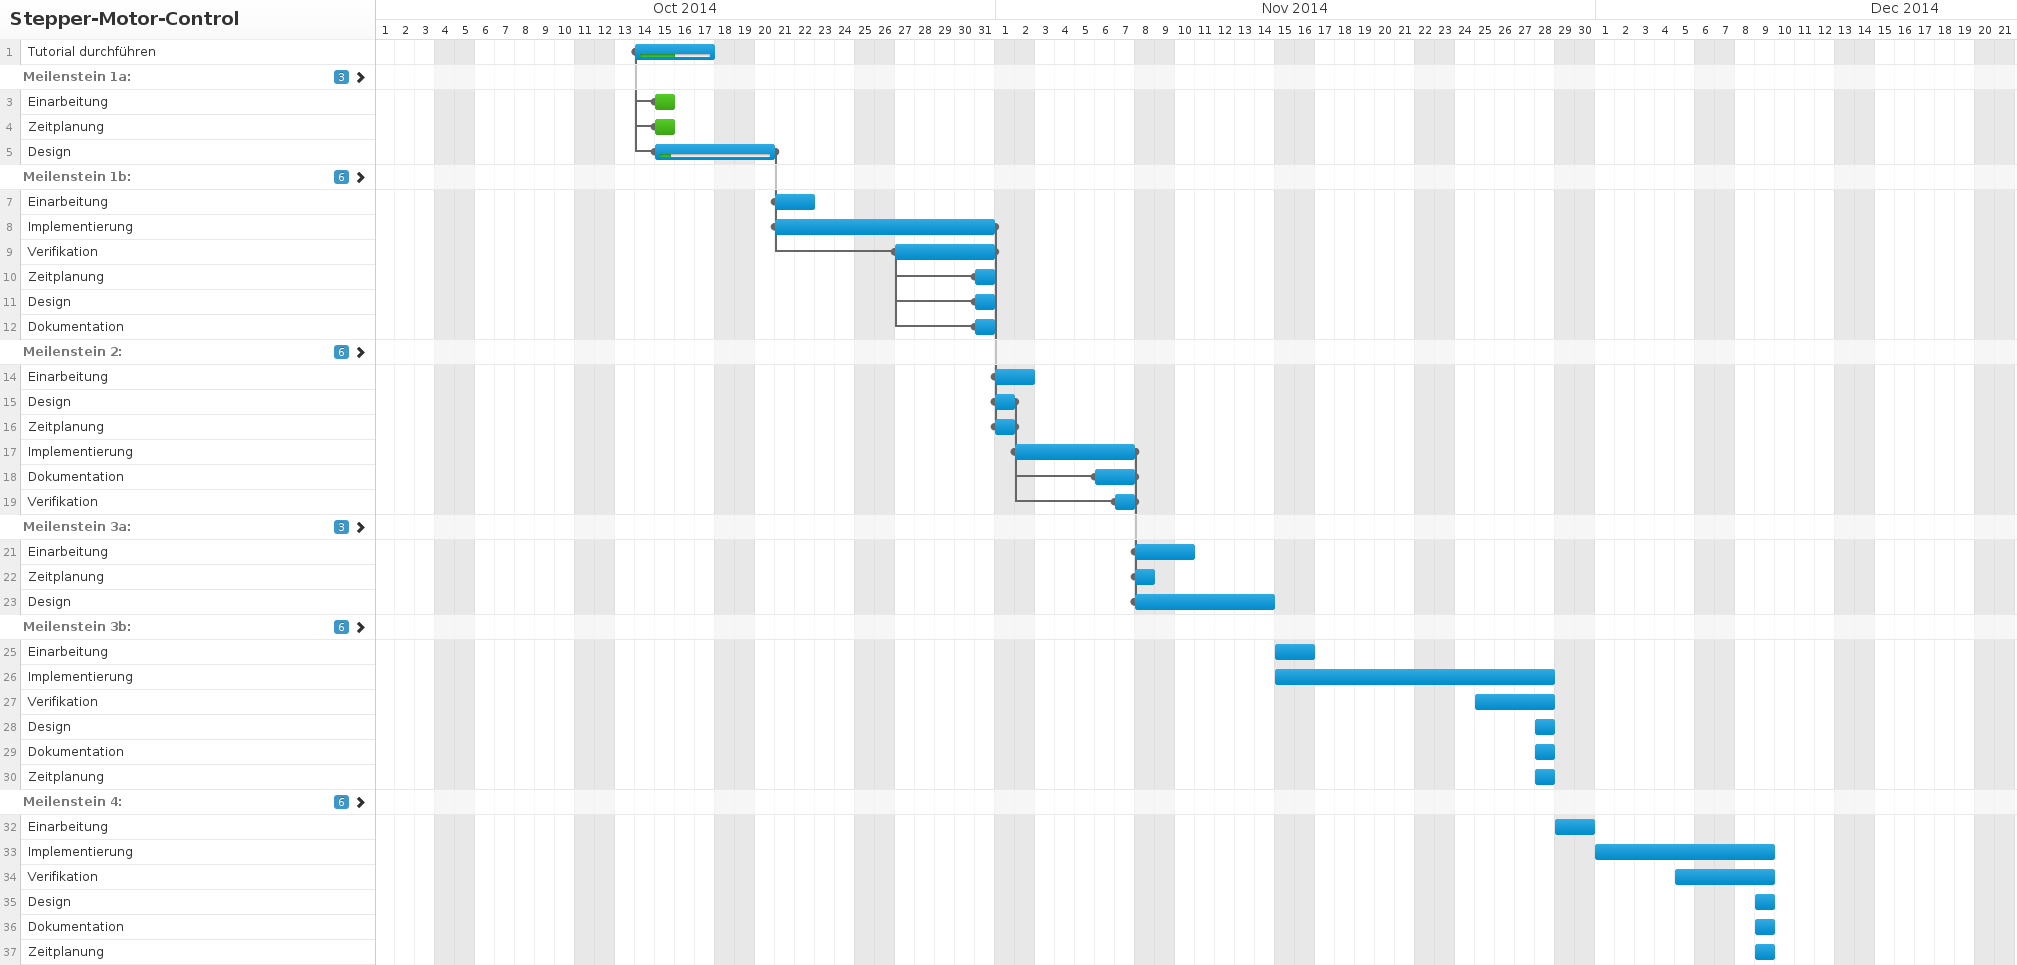
\includegraphics[scale=.3,angle=90]{../../Planning/Gantt-Diagramm.png}
\end{center}
\caption{Gantt-Diagramm zur kompletten Zeitplanung}
\label{fig:gantt}
\end{figure}

\begin{figure}[htbp]
\centering
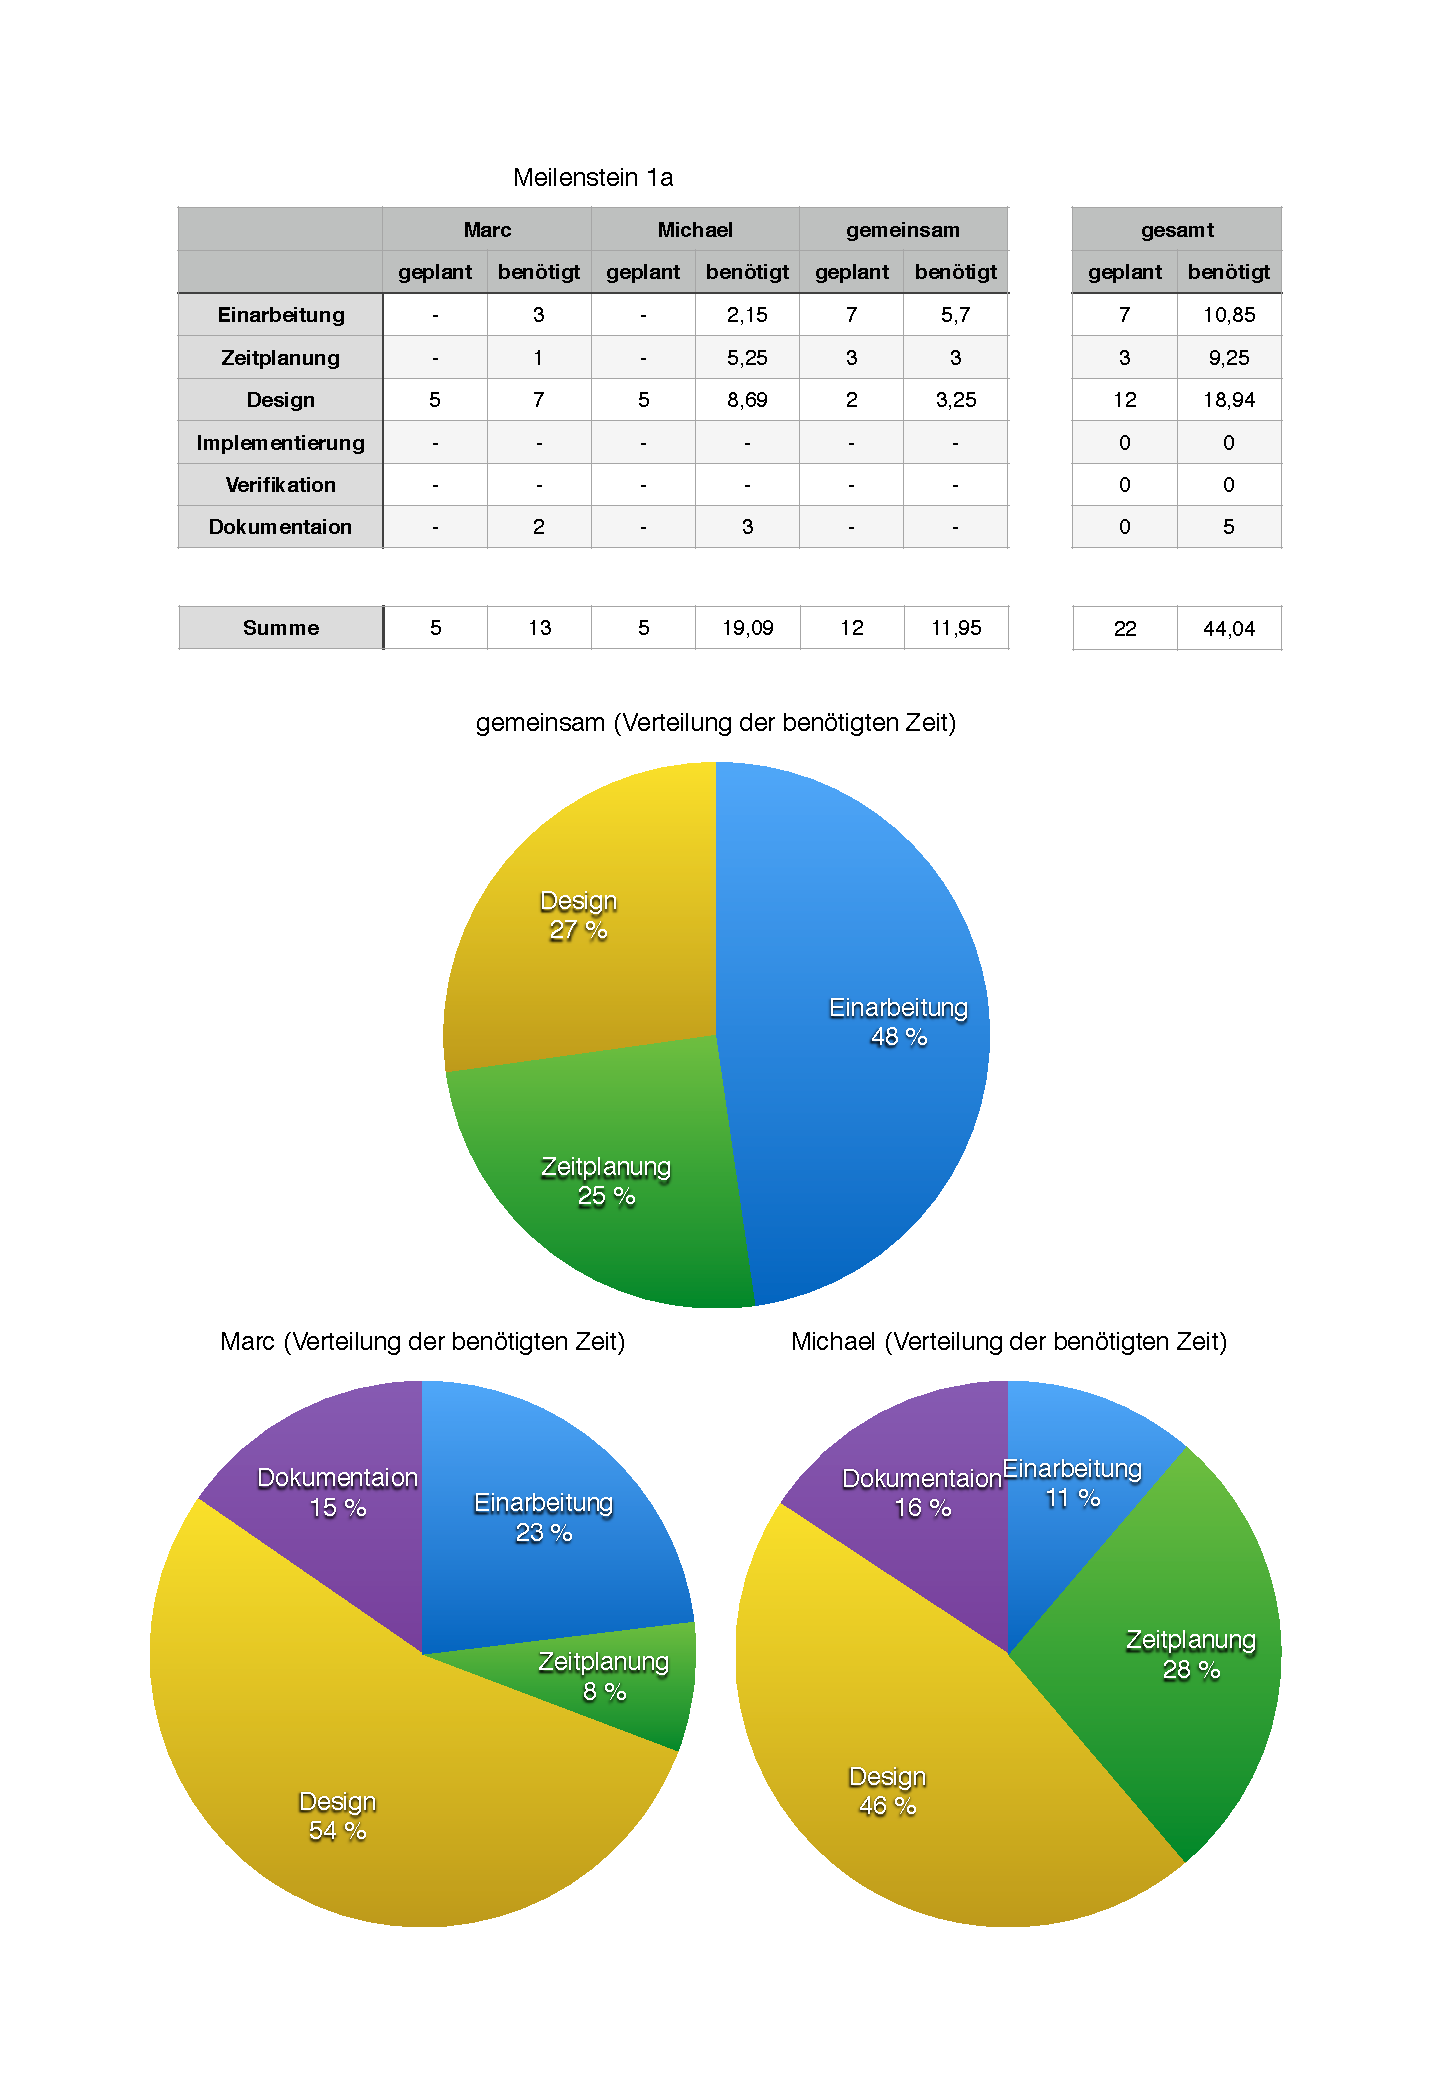
\includegraphics{../../Planning/Planung_Meilenstein1a.pdf}
\caption{Projektplanung für Meilenstein 1a\label{fig:projektplanung}}
\end{figure}

\begin{figure}[htbp]
\centering
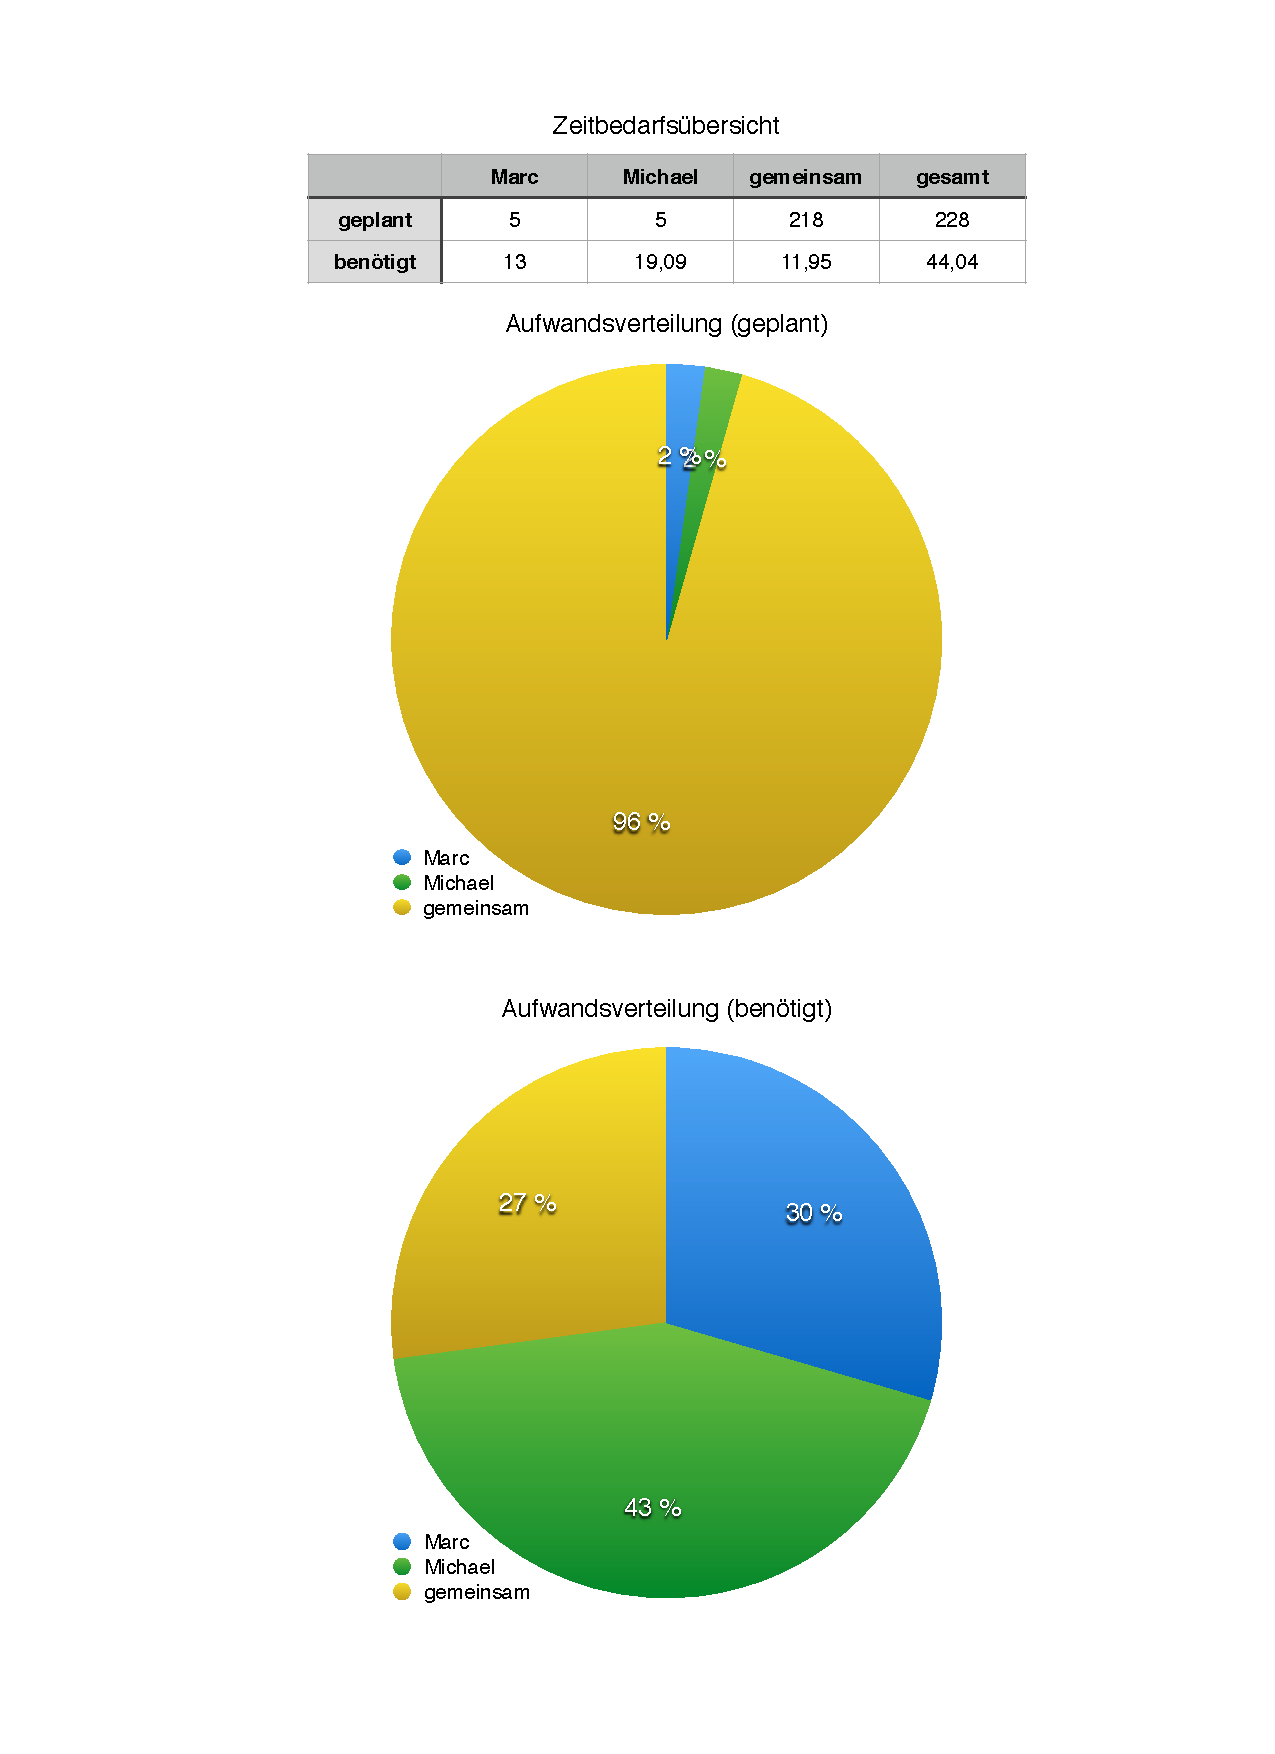
\includegraphics{../../Planning/Zeitbedarf.pdf}
\caption{Zeitbedarfsübersicht für das gesamte
Projekt\label{fig:zeitbedarf}}
\end{figure}

\newpage
\# Beschreibung der Anwendungsfälle

Gemäß Abbildung \ref{fig:anwendungsfaelle} hat der Anwender (dargestellt
als \emph{User}) die Möglichkeit, den Modus der Steuerung (\emph{mode}),
die Drehrichtung (\emph{direction}) und die Drehgeschwindigkeit
(\emph{speed}) einzustellen, sowie den Motor zu starten und zu stoppen
(\emph{start/stop motor}).

\begin{figure}[htbp]
\centering
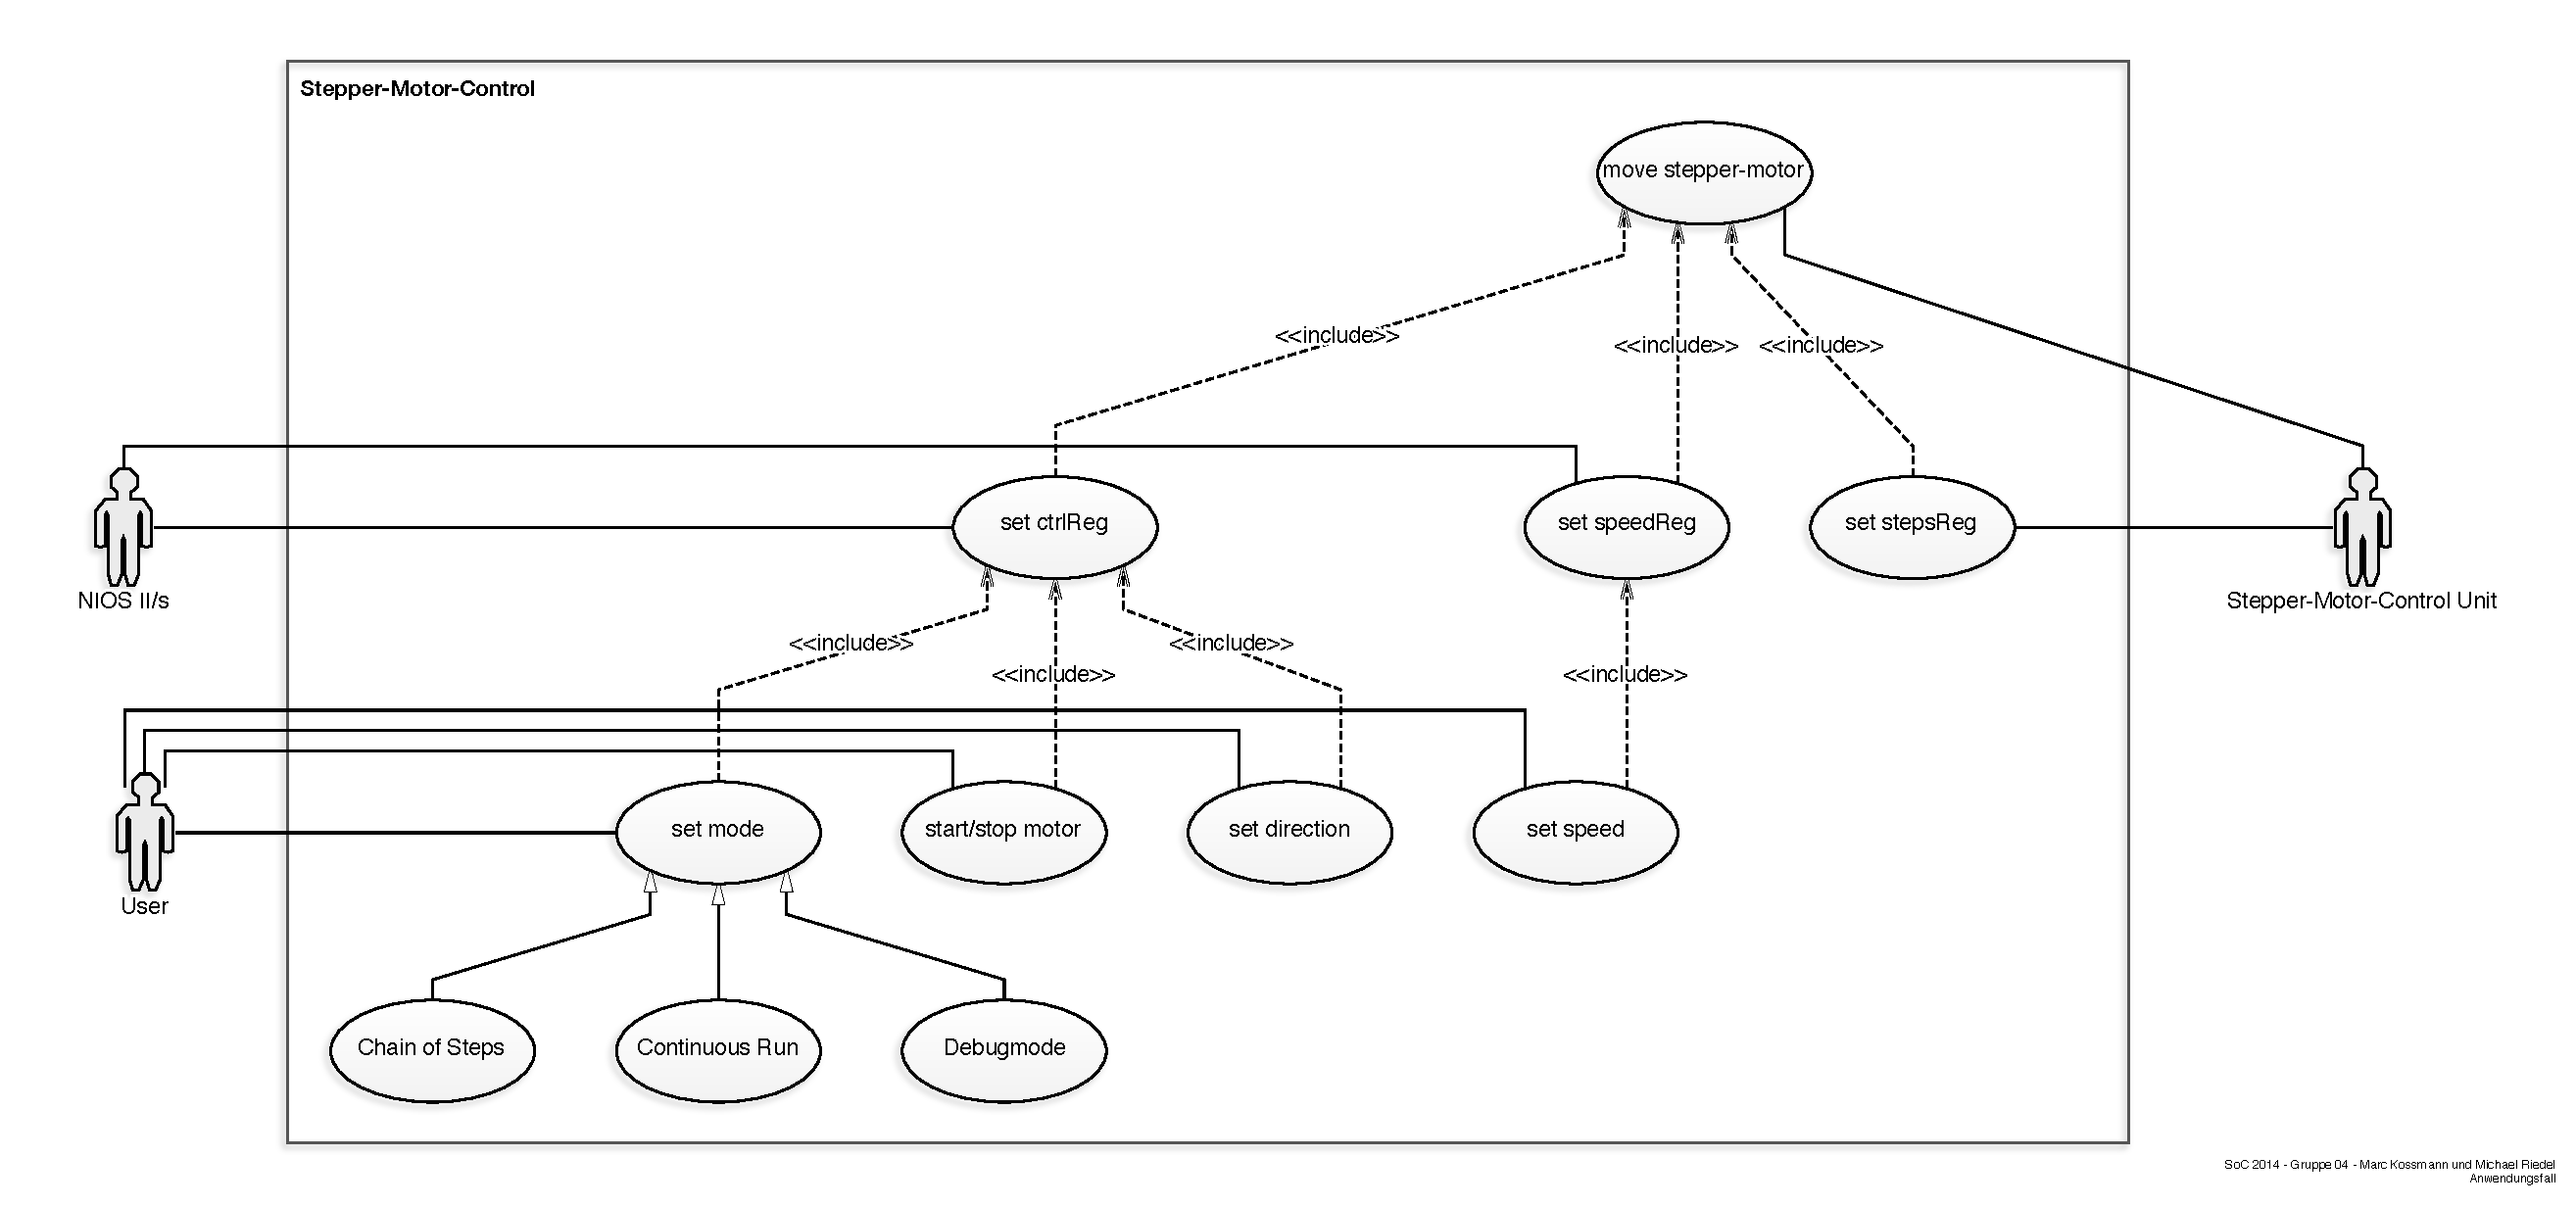
\includegraphics{../Diagrams/UseCases.pdf}
\caption{Anwendungsfälle\label{fig:anwendungsfaelle}}
\end{figure}

Der Anwender kann somit zwischen drei Modi wählen:

\begin{itemize}
\item
  \emph{Chain of Steps}: Dabei wird der Motor um eine fest angegebene
  Schrittweite mit gewählter Geschwindigkeit verfahren.
\item
  \emph{Continuous Run}: Dabei verfährt der Motor mit vorher
  eingestellter Geschwindigkeit, bis er durch den Anwender gestoppt
  wird.
\item
  \emph{Debugmode}: Im Debug-Modus wird in regelmäßigen Abständen der
  Motor bewegt, ein Interrupt ausgelöst und die Register verändert.
\end{itemize}

Entsprechend den Eingaben durch den Anwender, werden durch den NIOS
II/s-Prozessor die Register verändert und der Motor entsprechend durch
die \emph{Motor-Control-Unit (MCU)} verfahren.

\chapter{Beschreibung der benötigten Tasks und
Interrupt-Service-Routinen}\label{beschreibung-der-benuxf6tigten-tasks-und-interrupt-service-routinen}

Das Steuerprogramm zur Kontrolle des Schrittmotors reagiert auf Eingaben
durch den Benutzer. Dies geschieht über verschiedene Schalter und
Taster. Außerdem werden dem Benutzer während des Betriebs Informationen
über ein LC-Display, eine \emph{JTAG-UART Debug-Console} und LEDs
angezeigt. Die Steuerung des Motors geschieht über eine eigene MCU, die
anhand von in Registern abgelegten Informationen, bedient wird. Das
Steuerprogramm und die MCU kommunizieren somit nur über die zur
Verfügung stehenden Register und Interrupt-Leitungen.

\section{benötigte Tasks}\label{benuxf6tigte-tasks}

Damit Aufgaben parallel abgearbeitet werden können, werden drei Tasks
verwendet:

\subsection{Die Hauptsteuerung durch die
User-Input-Task}\label{die-hauptsteuerung-durch-die-user-input-task}

Die \enquote{Main-Task} oder auch \lstinline!User-Input-Task! stellt,
gemäß Abbildung \ref{fig:user_input}, die höchste Kontrollinstanz dar.
Nach der Initialisierung der Hardware, Interrupt-Service-Routinen (ISR)
und der Ausgabe von Systeminformationen auf dem Display und in der
\emph{JTAG-UART Debug-Console} gemäß Abbildung \ref{fig:init}, reagiert
die Steuersoftware des NIOS II/s-Prozessors auf eingehende
Benutzereingaben. Anhand derer werden, wenn nicht gerade der Motor
läuft, die entsprechenden Register verändert.

Wird der Taster \lstinline!Key 0! zum Starten des Motors gedrückt, so
wird ein letztes Mal der Modus überprüft, sodass die MCU mit den
Informationen der Register den Schrittmotor bewegen kann. Während der
Motor läuft, ist vom Steuerprogramm nur die Drehrichtung veränderbar.
Natürlich lässt sich der Schrittmotor jederzeit anhalten.

\subsection{Die Ausgabe durch die
User-Output-Task}\label{die-ausgabe-durch-die-user-output-task}

Eine eigene \lstinline!User-Output-Task! stellt, gemäß Abbildung
\ref{fig:user_output} dem Benutzer Informationen zur Verfügung. Sie
zeigt auf dem LC-Display neben der Programmversion, den Motormodus und
Motorstatus an. Außerdem ist bei eingeschaltetem \emph{Debug}-Modus dies
kenntlich gemacht. Weil im Display nicht alle Informationen
übersichtlich dargestellt werden können, werden zusätzlich die
HEX-Anzeigen 0 bis 2 zur Anzeige der Drehrichtung, der Geschwindigkeit
und es Modus benutzt.

Währenddessen werden in einem über die JTAG-UART-Schnittstelle
angeschlossenen Terminal Meldungen dargestellt. Diese enthalten alle
Inhalte der Register zur Kommunikation mit der MCU.

\subsection{Die Heartbeat und
Debug-Task}\label{die-heartbeat-und-debug-task}

Eine Forderung an die Steuersoftware ist die Anzeige eines
\emph{Heartbeats}. Damit lässt sich gemäß Abbildung
\ref{fig:heartbeat_debug} jederzeit erkennen, ob der Prozessor noch in
einem funktionsfähigen Betriebszustand ist. Dieser Heartbeat wird über
eine eigene Task namens \lstinline!Heartbeat-Task! erzeugt und auf der
HEX-Anzeige 3 und der LED 9 durch einen Blinkcode dargestellt.

Wenn der \emph{Debug-Schalter} auf \lstinline!1! gestellt wurde, wird in
der \emph{Heartbeat}-Task alle 3 Sekunden ein Interrupt erzeugt, das dem
Steuerprogramm das Anhalten des Motors signalisiert. Wenn das
\lstinline!Run-Bit! im Control-Register (\lstinline!ctrlReg!) auf
\lstinline!1! gesetzt ist, sich der Schrittmotor also dreht, wird
entsprechend der Drehrichtung das Register \lstinline!stepsReg! zum
zählen der Schritte verändert. So lässt sich das Programm ohne MCU
testen.

\section{benötigte
Interrupt-Service-Routinen}\label{benuxf6tigte-interrupt-service-routinen}

Um eine schnelle Interaktion mit der Schrittmotorsteuerung durch den
Anwender zu ermöglichen, werden drei ISR verwendet:

\subsection{Die Abfrage der Taster}\label{die-abfrage-der-taster}

Damit eine Reaktion auf Benutzereingaben in Echtzeit möglich ist, werden
die Taster gemäß Abbildung \ref{fig:key_isr} über eine
\lstinline!Key-ISR! ausgewertet. Sobald ein Taster gedrückt wurde, wird
der Interrupt gesetzt und im \emph{Interrupthandler} der Zustand der
Taster abgefragt. Für den gedrückten Taster wird dann ein \emph{Flag} an
die Main-Task gesetzt.

\subsection{Die Abfrage der Schalter}\label{die-abfrage-der-schalter}

Die \lstinline!Switch-ISR! reagiert gemäß Abbildung \ref{fig:switch_isr}
auf Änderungen der Schalterstellungen. Zur Einsparung von Flags werden
die Schalter etwas anders ausgewertet. Bei Betätigung wird auch ein
Interrupt ausgelöst, allerdings wird im \emph{Interrupthandler} die
Stellung aller Schalter in einer \emph{MessageQueue}-Variable
abgespeichert und anschließend nur ein \lstinline!Switch-Update-Flag! an
die Main-Task gesetzt. Diese muss dann die Schalterstellungen aus der
Queue abholen.

\subsection{Die Abfrage der
Motorsteuerung}\label{die-abfrage-der-motorsteuerung}

Zu guter Letzt wird gemäß Abbildung \ref{fig:motor_isr} über die
\lstinline!Motor-ISR! das Stoppen des Motors in der
\lstinline!Chain of Steps!-Betriebsart signalisiert. Im
\emph{Interrupthandler} wird nur ein Flag an die Main-Task gesendet.
Diese ISR ist mit dem \lstinline!IR!-Bit des Control-Registers
(\lstinline!ctrlReg!) verbunden.

\section{Darstellung der
Aktivitätsdiagramme}\label{darstellung-der-aktivituxe4tsdiagramme}

\begin{figure}[htbp]
\centering
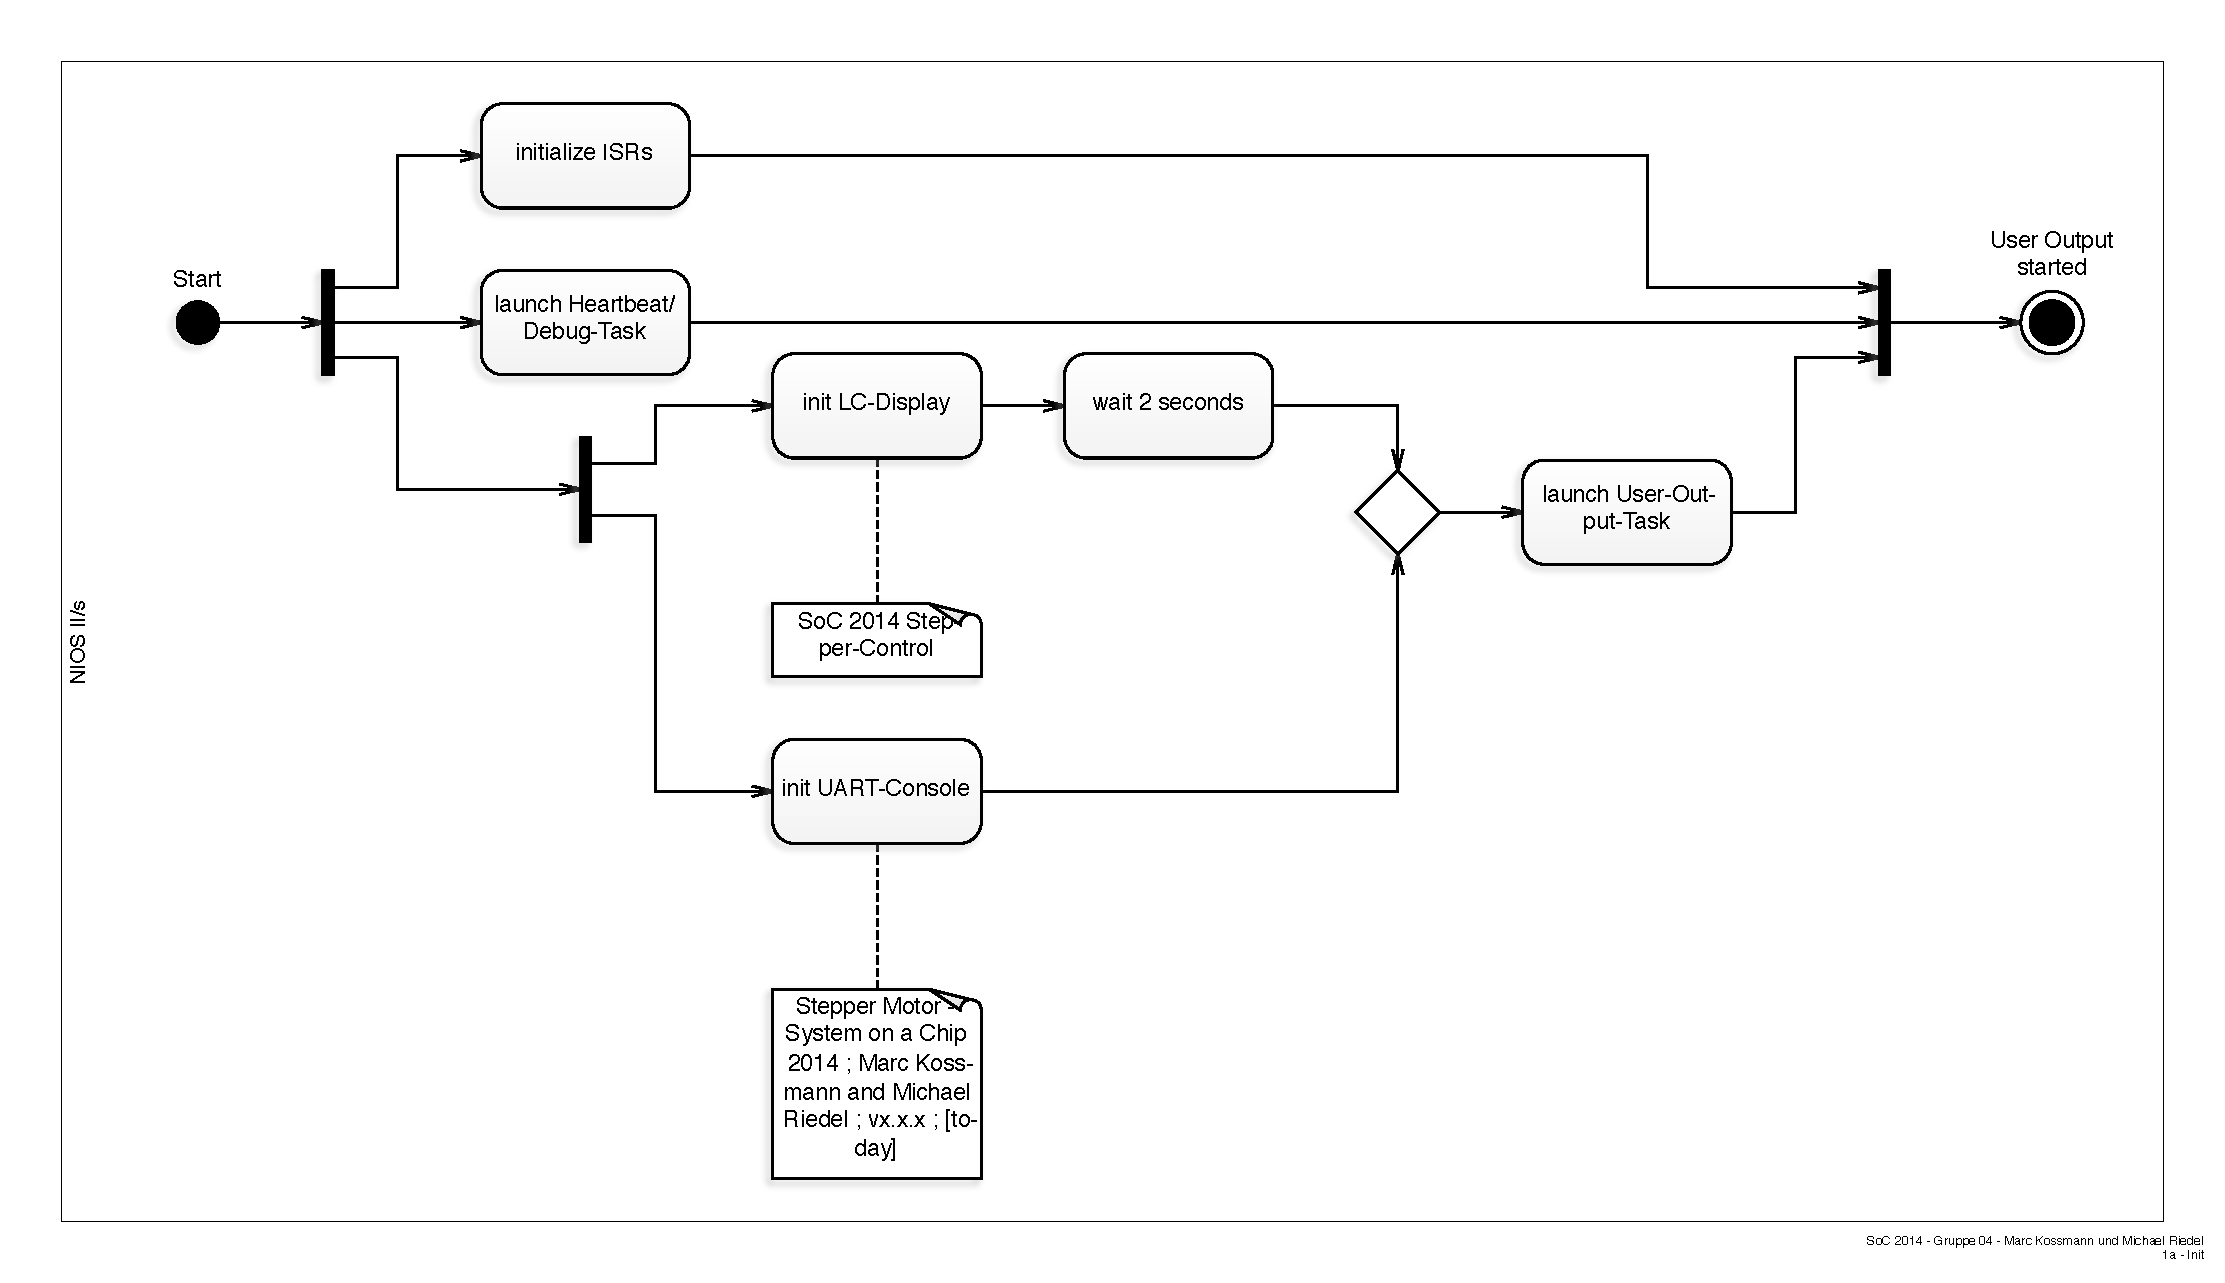
\includegraphics{../Diagrams/Activities/Functions/Init.pdf}
\caption{Initialisierung der Hardware, ISR und Tasks\label{fig:init}}
\end{figure}

\begin{figure}[htbp]
\centering
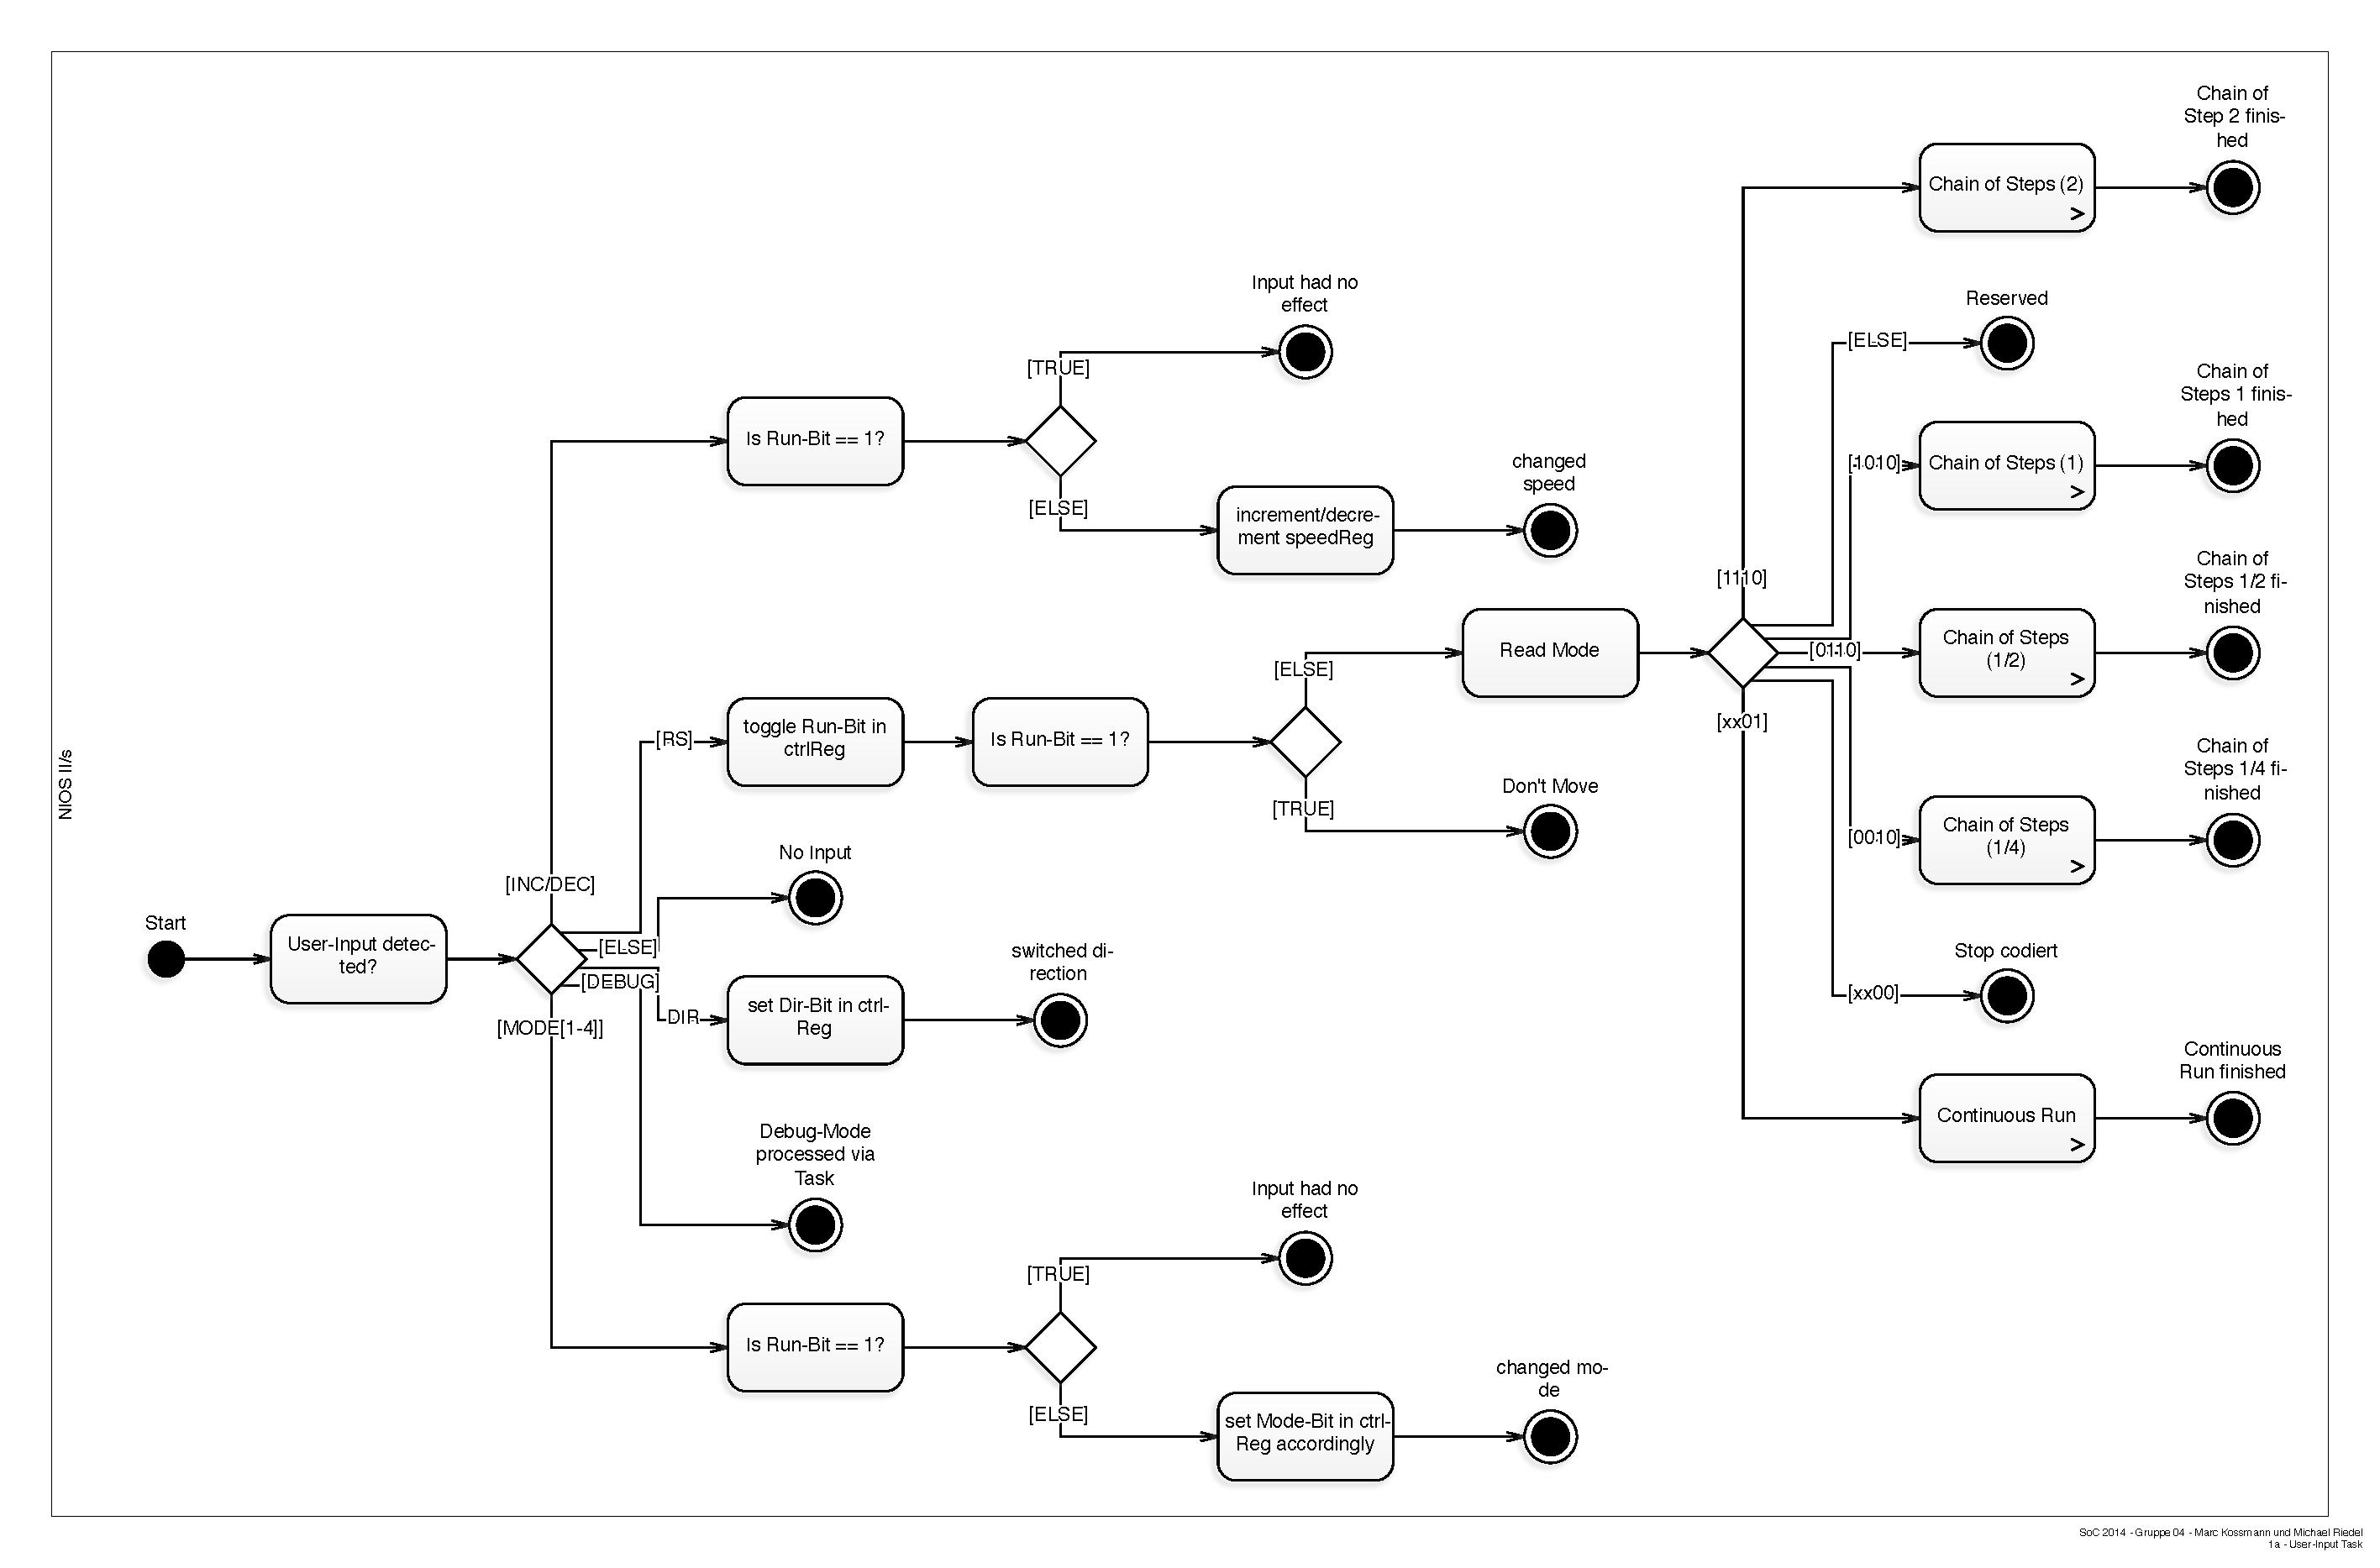
\includegraphics{../Diagrams/Activities/Tasks/User-Input.pdf}
\caption{User-Input Task\label{fig:user_input}}
\end{figure}

\begin{figure}[htbp]
\centering
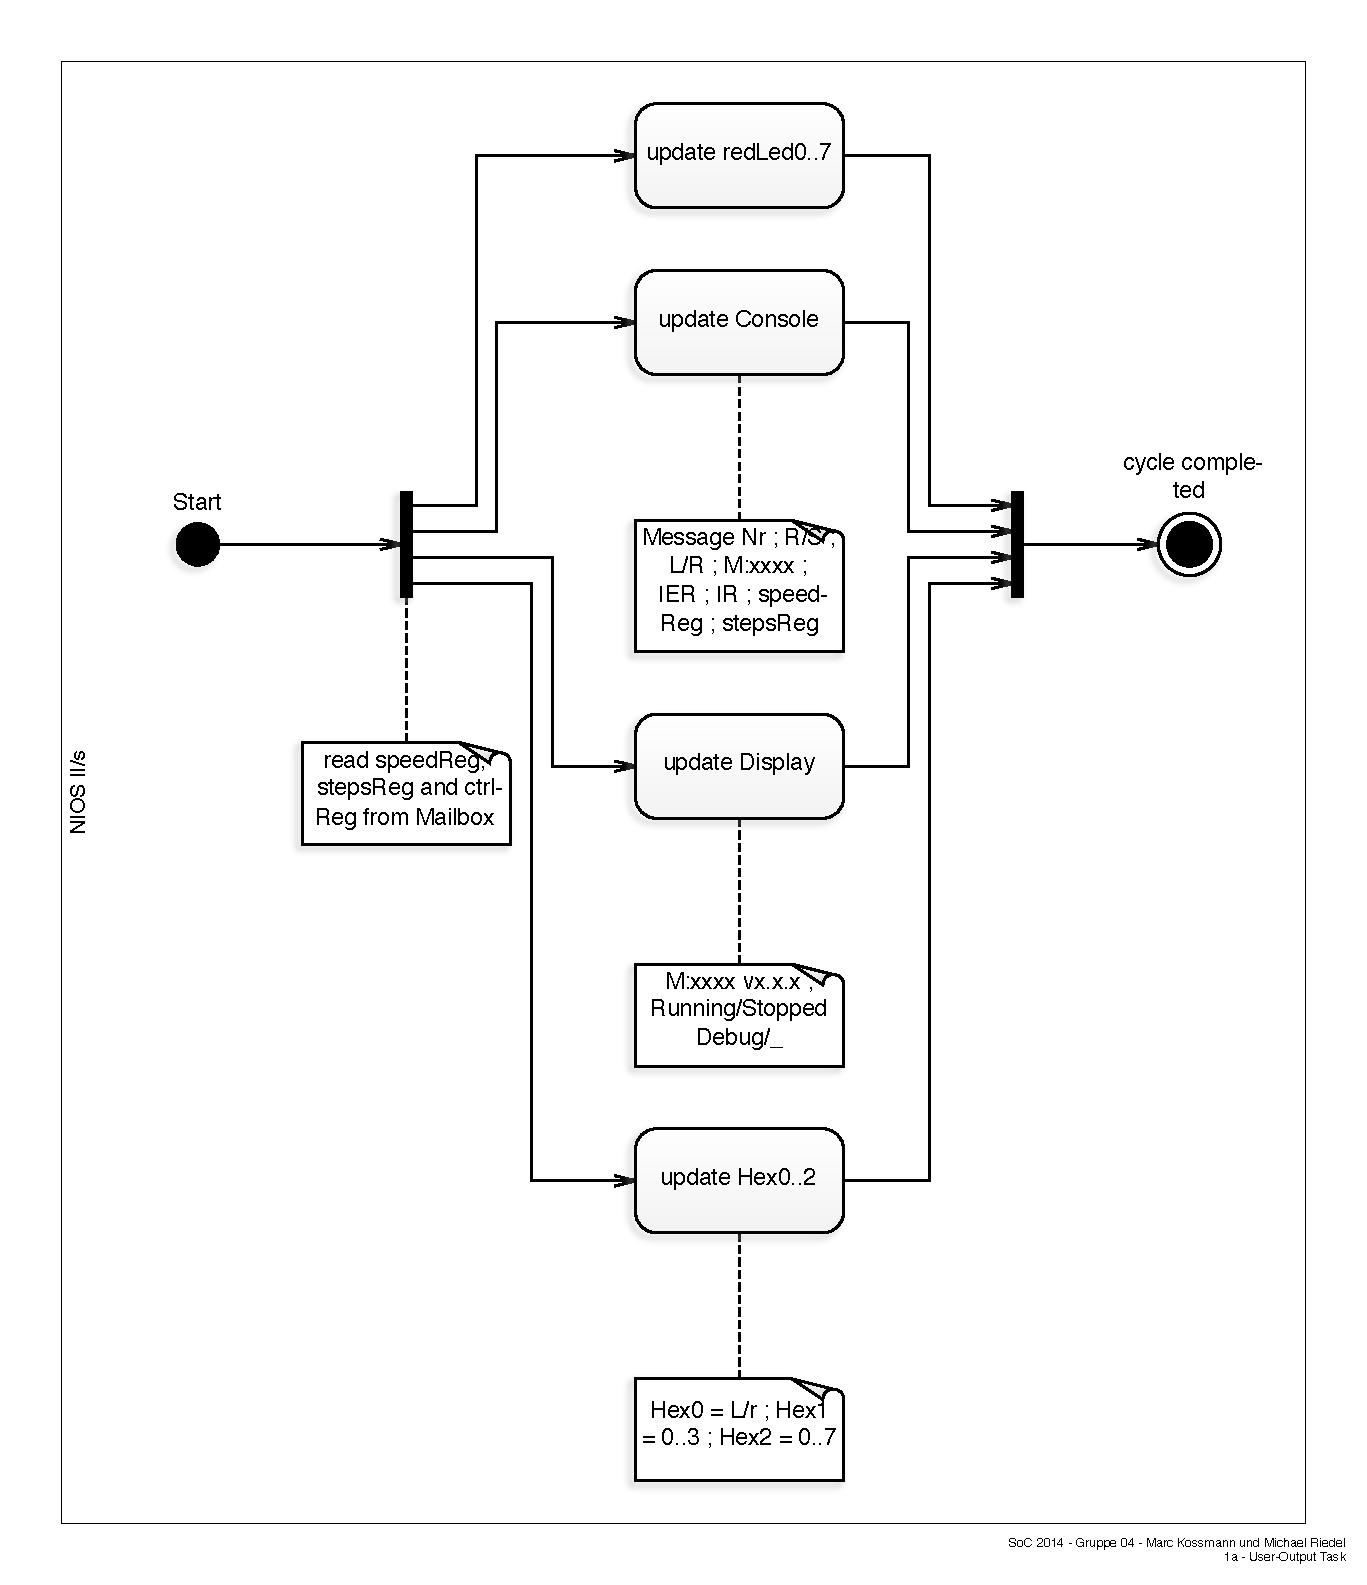
\includegraphics{../Diagrams/Activities/Tasks/User-Output.pdf}
\caption{User-Output Task\label{fig:user_output}}
\end{figure}

\begin{figure}[htbp]
\centering
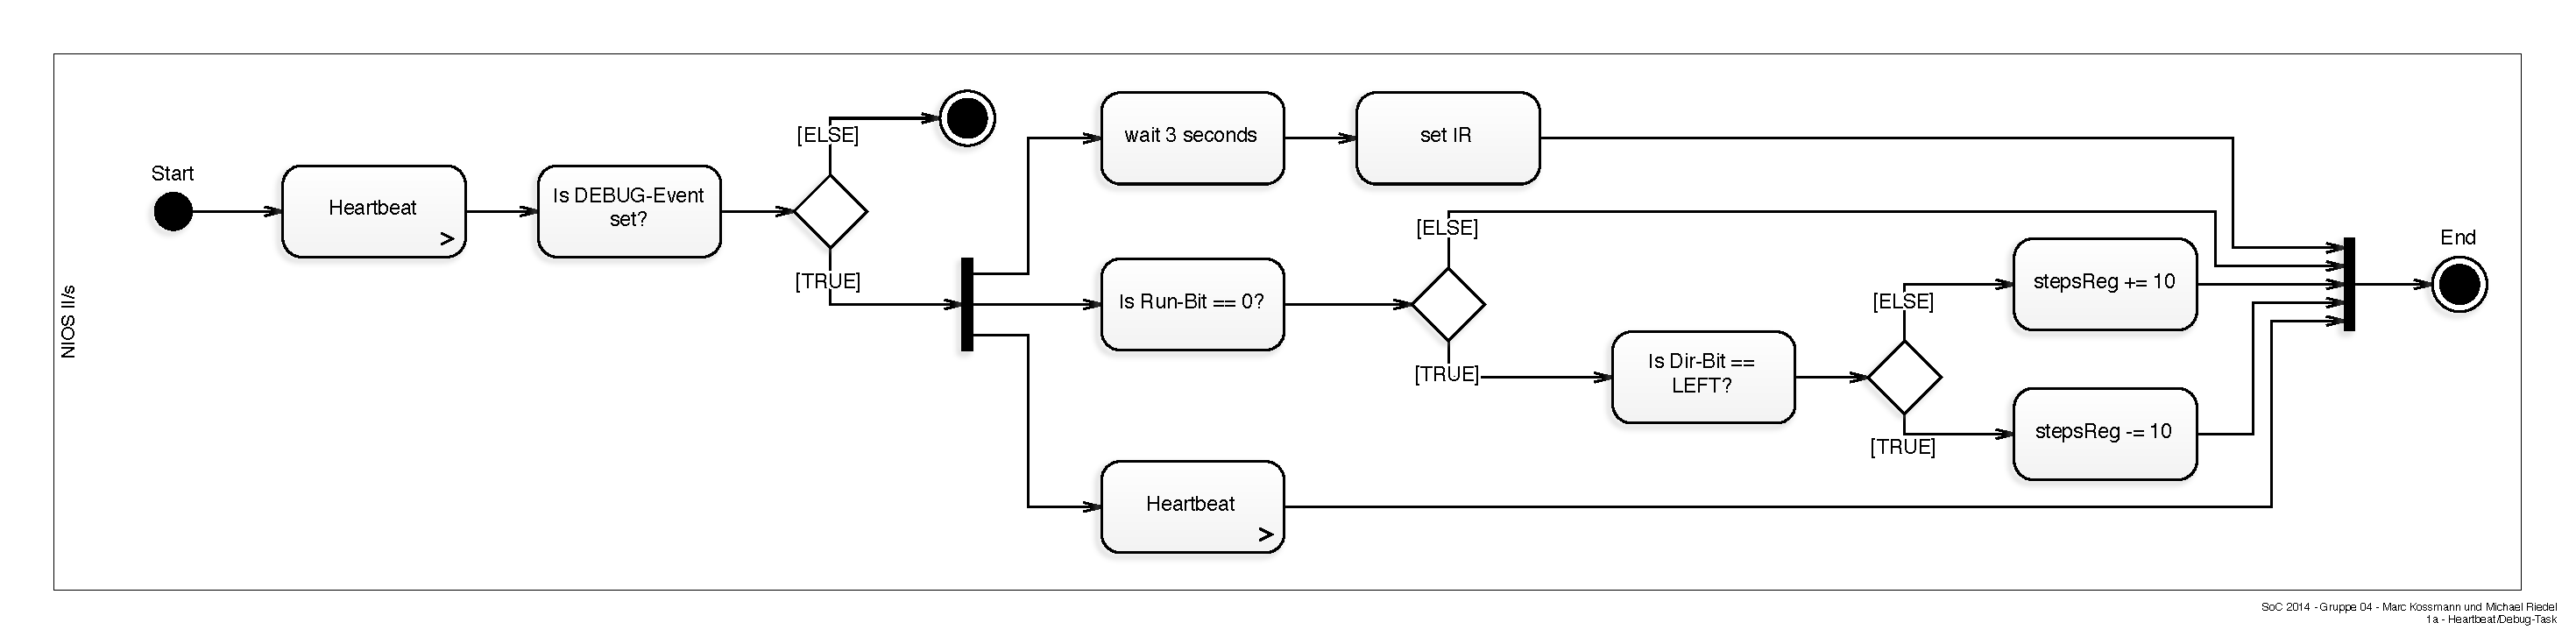
\includegraphics{../Diagrams/Activities/Tasks/Heartbeat-Debug.pdf}
\caption{Heartbeat-Debug Task\label{fig:heartbeat_debug}}
\end{figure}

\newpage

\begin{figure}[htbp]
\centering
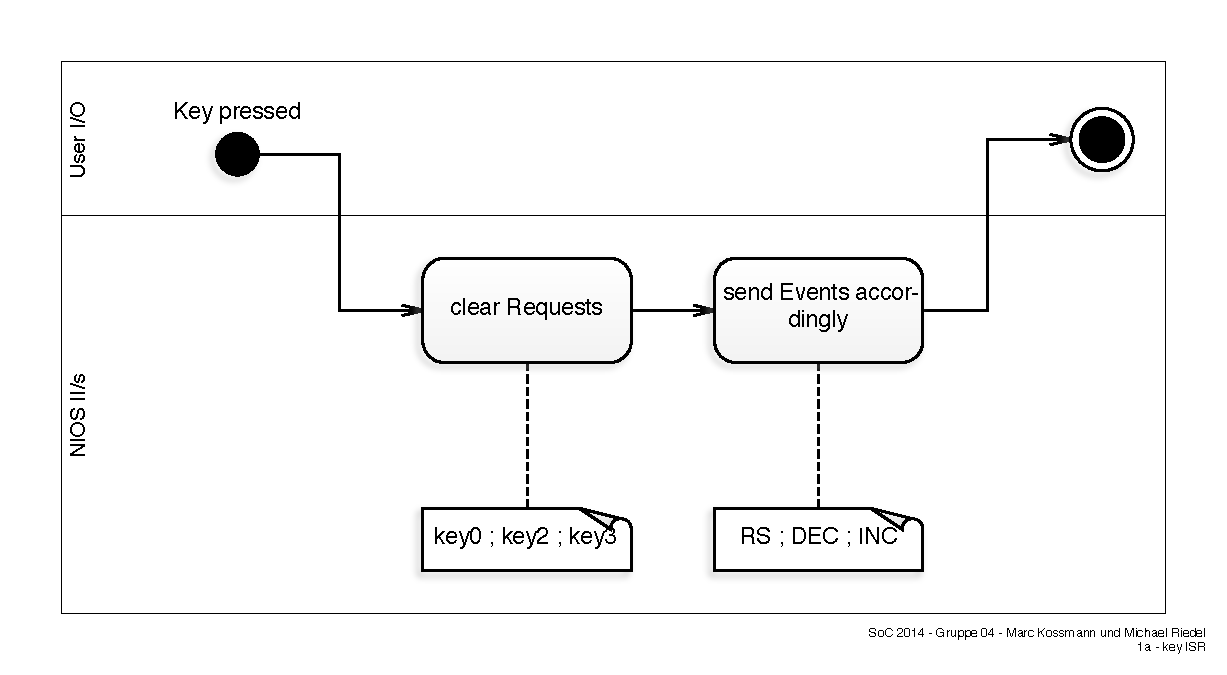
\includegraphics{../Diagrams/Activities/ISR/key_ISR.pdf}
\caption{Key ISR\label{fig:key_isr}}
\end{figure}

\begin{figure}[htbp]
\centering
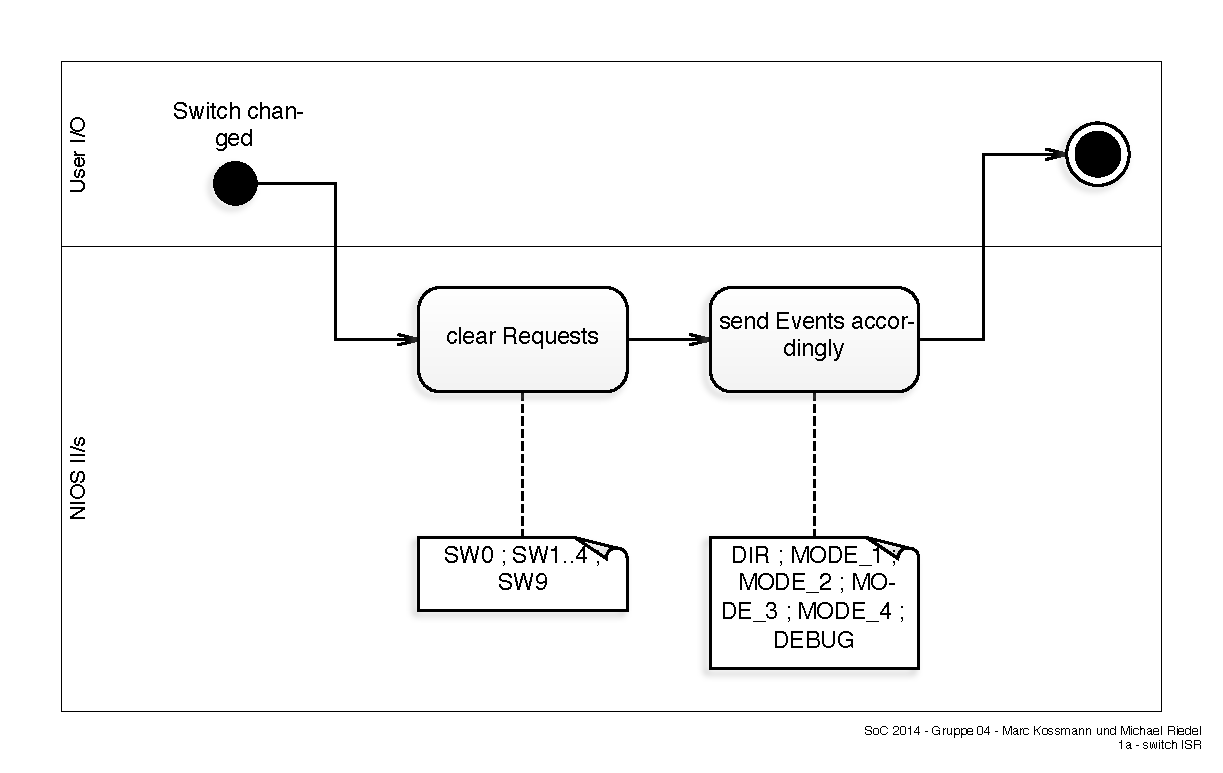
\includegraphics{../Diagrams/Activities/ISR/switch_ISR.pdf}
\caption{Switch ISR\label{fig:switch_isr}}
\end{figure}

\begin{figure}[htbp]
\centering
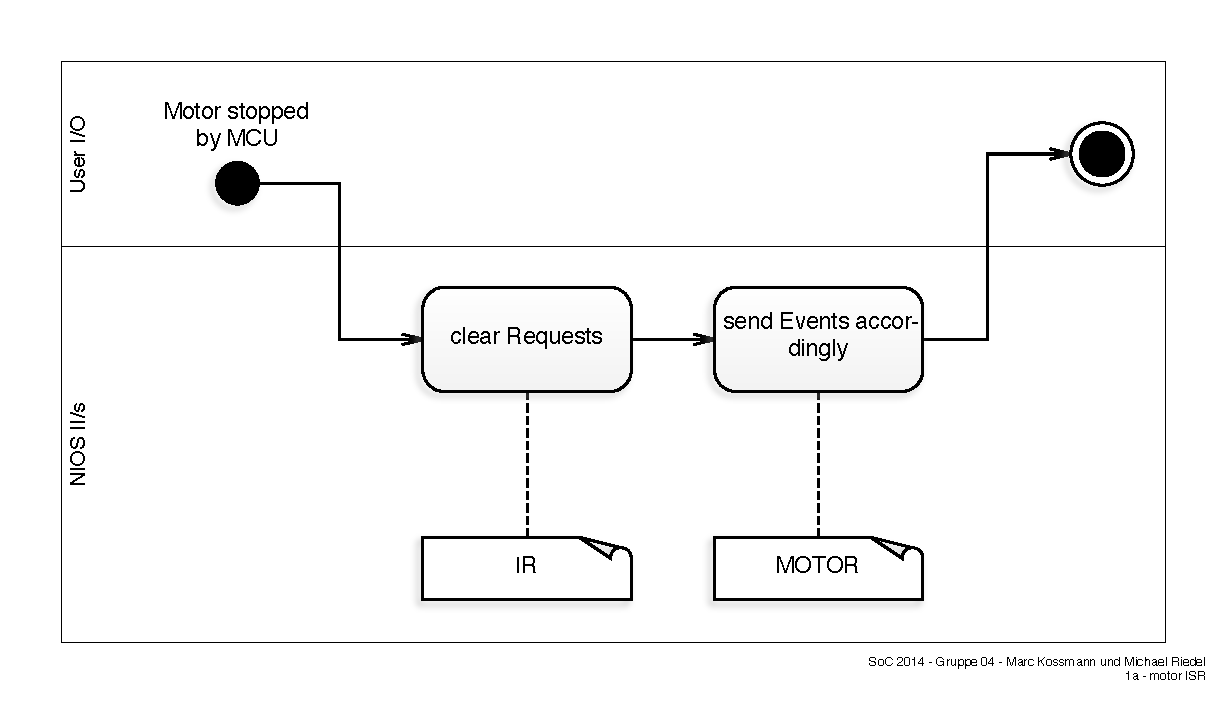
\includegraphics{../Diagrams/Activities/ISR/motor_ISR.pdf}
\caption{Motor ISR\label{fig:motor_isr}}
\end{figure}

\newpage

\begin{figure}[htbp]
\centering
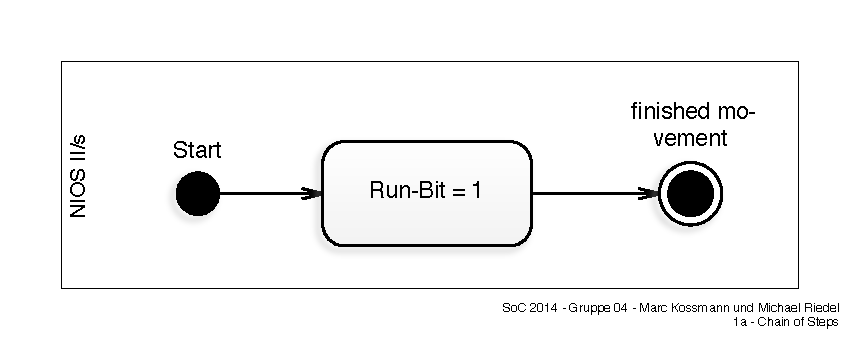
\includegraphics{../Diagrams/Activities/Functions/Chain-of-Steps.pdf}
\caption{Chain of Steps Funktion\label{fig:chain_of_steps}}
\end{figure}

\begin{figure}[htbp]
\centering
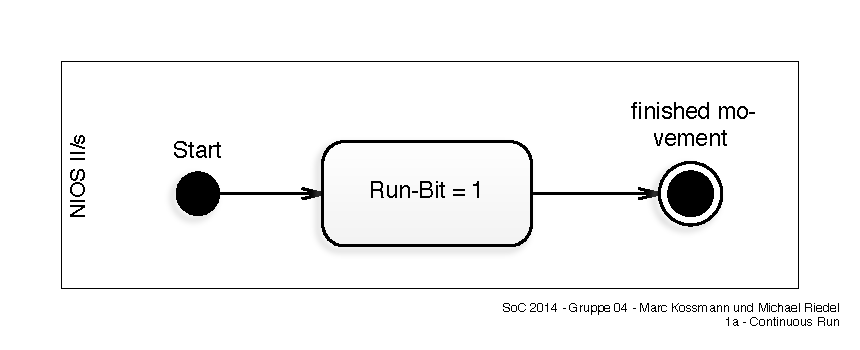
\includegraphics{../Diagrams/Activities/Functions/Continuous-Run.pdf}
\caption{Continuous Run Funktion\label{fig:continuous_run}}
\end{figure}

\begin{figure}[htbp]
\centering
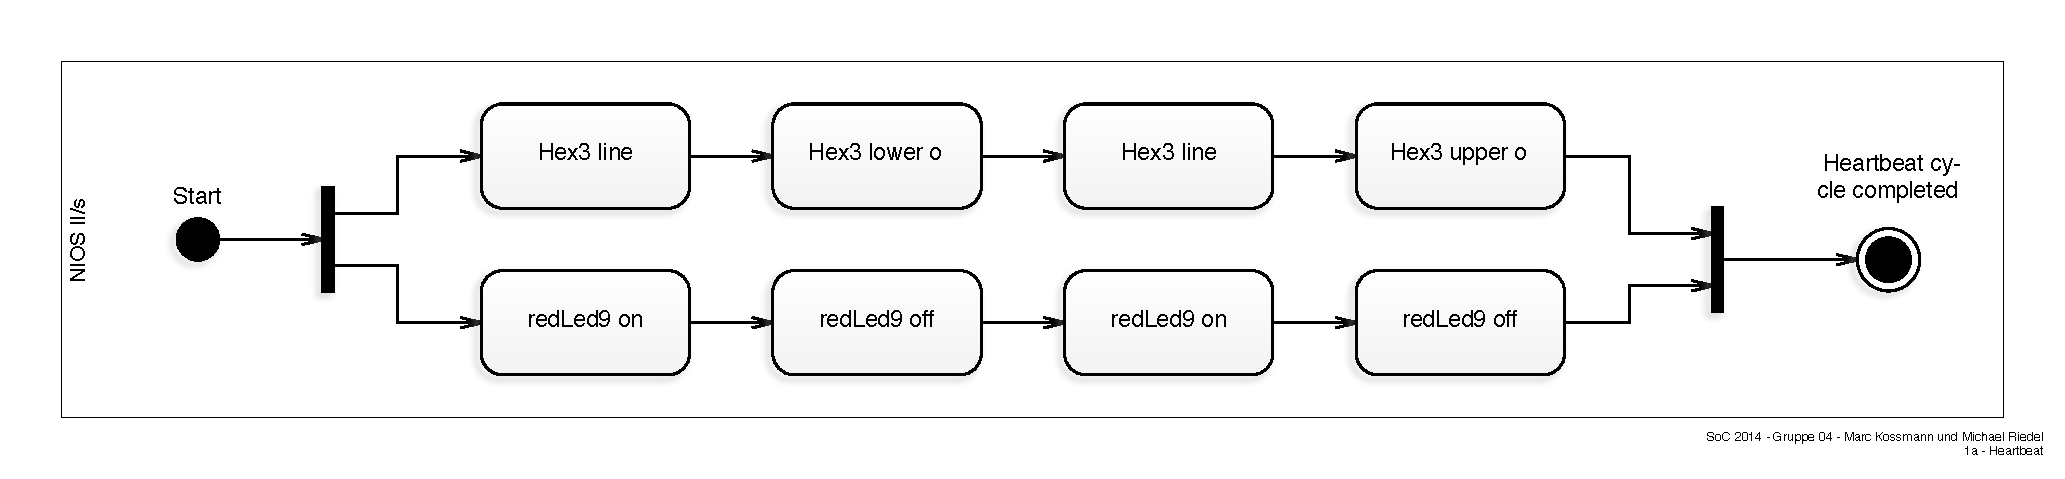
\includegraphics{../Diagrams/Activities/Functions/Heartbeat.pdf}
\caption{Heartbeat Funktion\label{fig:heartbeat}}
\end{figure}

\newpage

\chapter{Weitere Darstellungen zur Erläuterung der internen
Kommunikation}\label{weitere-darstellungen-zur-erluxe4uterung-der-internen-kommunikation}

\begin{figure}[htbp]
\centering
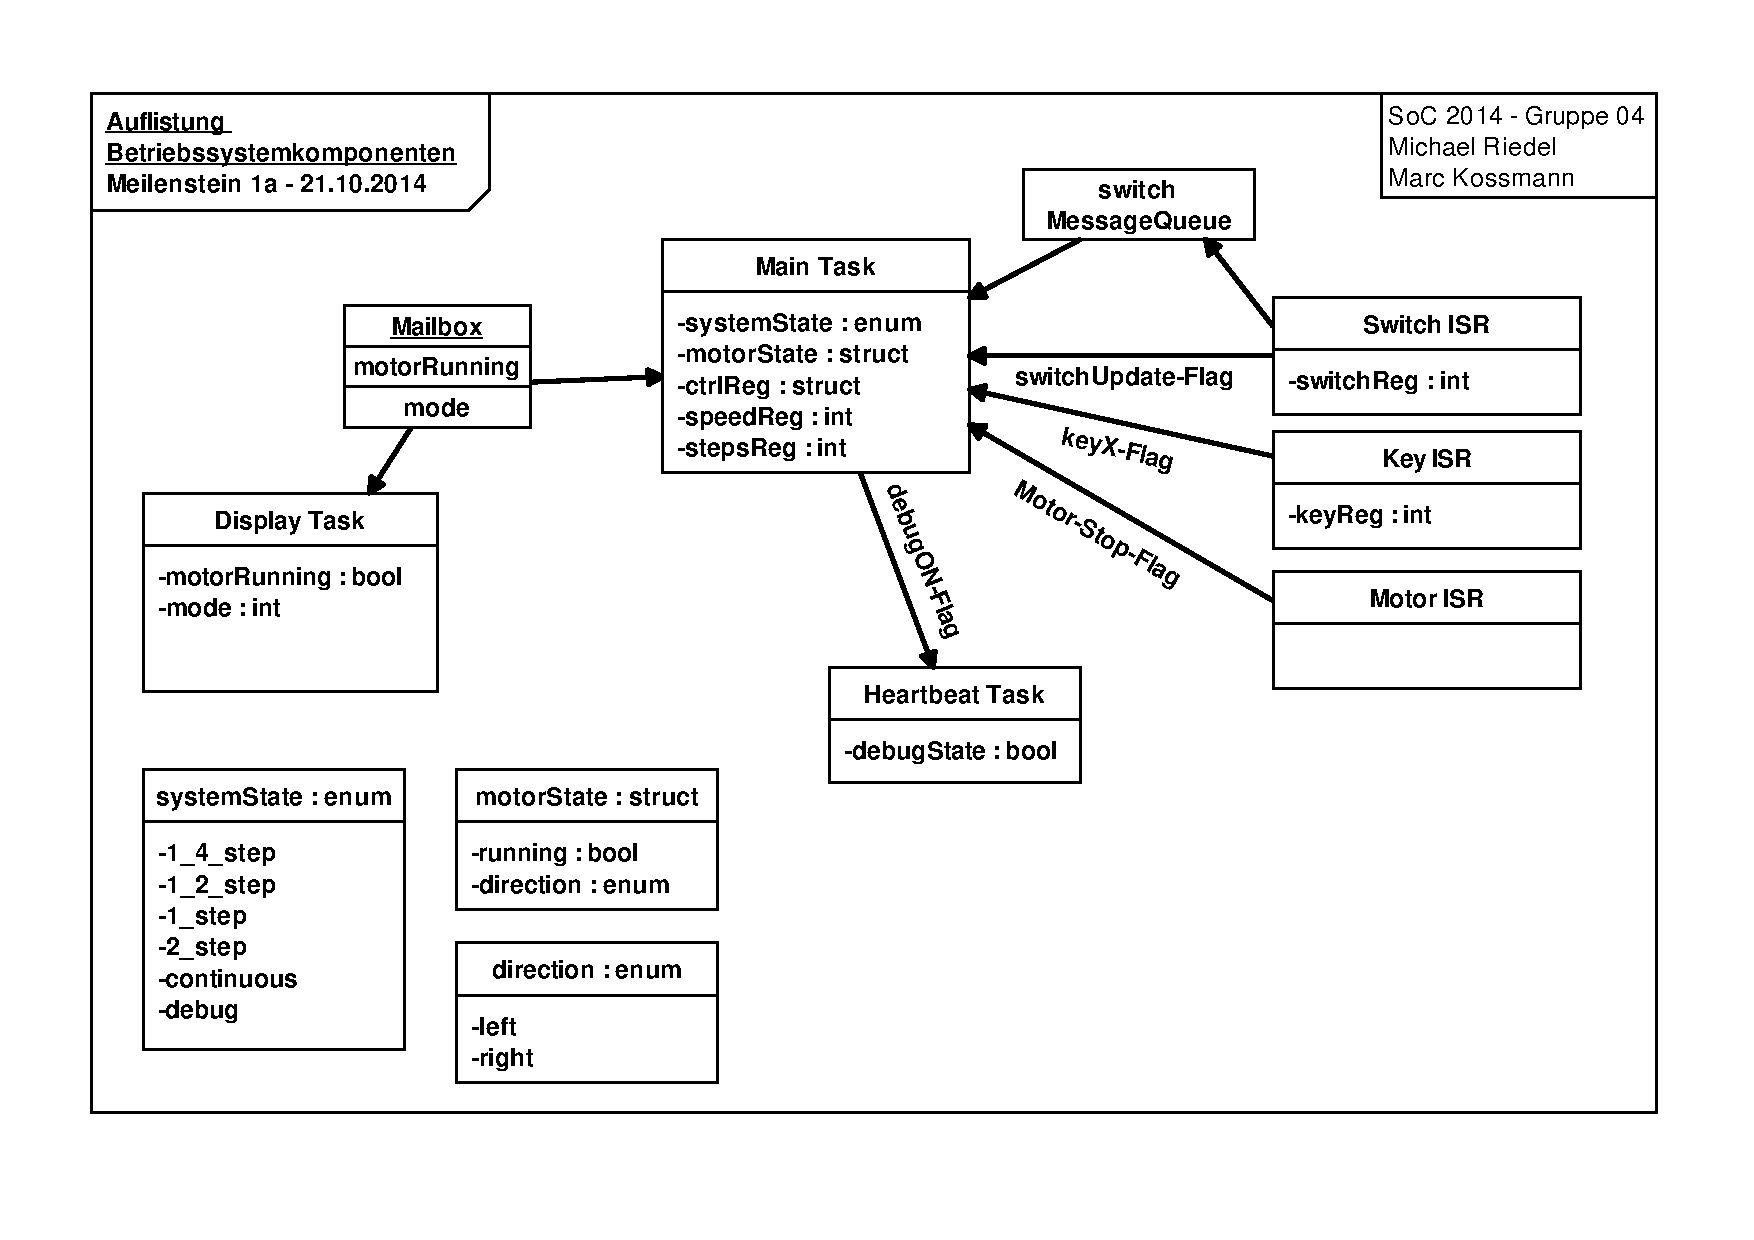
\includegraphics{../Diagrams/Auflistung_Betriebssystemkomponenten.pdf}
\caption{Auflistung Betriebssystemkomponenten\label{fig:auflistung}}
\end{figure}

\begin{figure}[htbp]
\centering
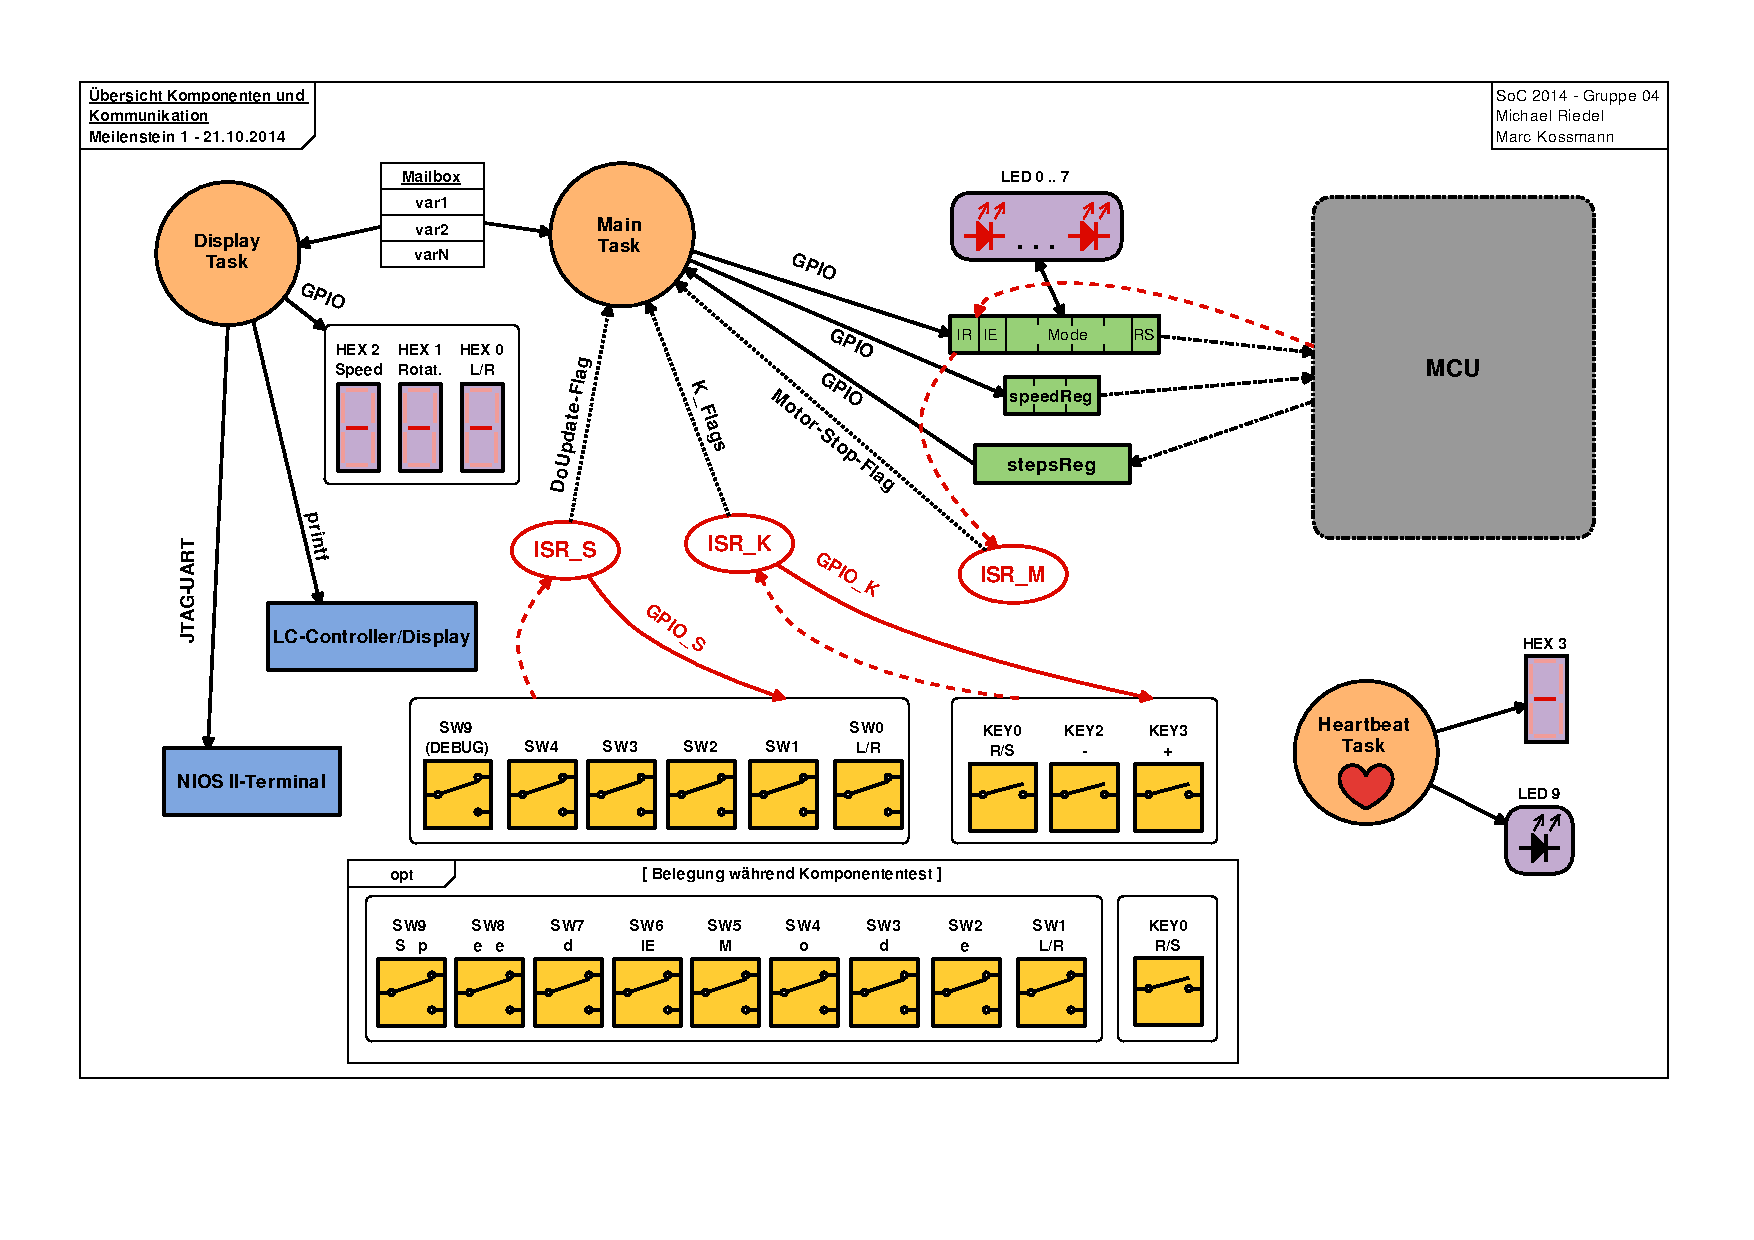
\includegraphics{../Diagrams/Uebersicht_Komponenten_und_Kommunikation.pdf}
\caption{Übersicht der Komponenten und
Kommunikation\label{fig:kommunikation}}
\end{figure}

\newpage

%%%%%%%%%%%%%%
% BACKMATTER %
%%%%%%%%%%%%%%
\ifthenelse{\equal{scrbook}{scrbook}}
  {
    \backmatter
  }{}


\pagenumbering{Roman}

% Print every collections
\printnoidxglossary[style=list_auto,title=Abkürzungsverzeichnis]
\newpage
\ifthenelse{\equal{true}{true}}
{
  \listoffigures
}{}
\ifthenelse{\equal{}{true}}
{
  \listofalgorithms
}{}
\ifthenelse{\equal{}{true}}
{
  \listoflistings
}{}
\ifthenelse{\equal{}{true}}
{
  \listoftables
}{}
\newpage


\end{document}